\chapter{Utilizzo}
Nei prossimi punti vediamo degli accorgimenti che sono utili per far utilizzare il sistema nel modo corretto. Per osservare degli esempi di come strutturare il codice osservare le sezioni di questo capitolo.
\begin{itemize}
    \item Gli elementi del sistema, come chunk, task, taskset, scheduler e protocollo di accesso alle risorse, devono essere definiti all'interno del main. Una volta definito tutto si deve chiamare il metodo \texttt{schedule} sullo scheduler. Nel caso si voglia generare una sorta di dataset di tracce, è prevista la possibilità di chiamare più volte il metodo \texttt{schedule} all'interno dello stesso main. Per generare un dataset di tracce è invece necessario chiamare il metodo \texttt{scheduleDataset} passando come parametro il numero di tracce.
    \item Un chunk campiona il suo tempo di esecuzione da una distribuzione. Tale distribuzione, passata come parametro del costruttore, è un oggetto di tipo \texttt{Sampler} definito nella libreria Sirio. Oltre alle distribuzioni introdotte da Sirio è presente anche l'implementazione \texttt{ConstantSampler}, che definisce un campionamento costante.
    \item I tempi devono essere passati al sistema e letti da esso in millisecondi. Il sistema li gestisce in nanosecondi per avere un'alta precisione.
    \item Quando si vuole introdurre il fault relativo alla priorità dinamica settata da PCP si deve specificare il valore minimo e massimo entro cui campionare. Questi valori sono intesi come esclusi.
    \item Quando si vuole introdurre il fault relativo all'acquisizione del semaforo associato alle risorse, la soglia specificata deve essere in un intervallo tra 0.0 e 1.0.
\end{itemize}
Per concludere analizziamo come il sistema si comporta sulla generazione di dataset. Si procederà in modo incrementale, per capire come affrontare lo scheduling di taskset più semplici e poi quelli più complessi.

Questa parte può essere anche utile per capire come strutturare il main ed utilizzare il simulatore.

%%%%%%%%%%%%%%%%%%%%%%%%%%%%%%%%%%%%%%%%%%%%%%%%%%%%%%%%%%%%%%%%
\section{Baseline}
Vediamo come funziona una simulazione tramite RM con un taskset molto semplice. Il taskset in questione, come si può notare dal codice in Figura~\ref{fig:baselineTaskset}, è molto semplice in modo da poter osservare le differenze tra le due simulazioni. Si tratta di un taskset con due task puramente periodici: il primo ha periodo e deadline relativo pari a 20ms e un chunk con un execution time di 10ms; il secondo ha periodo e deadline di 60ms e tre chunk con execution time rispettivamente di 5ms, 4ms e 3ms.

La traccia in Figura~\ref{fig:baselineTrace} è l'output della simulazione.

\begin{figure}[htbp]
    \centering
    \begin{subfigure}{0.45\textwidth}
        \vfill
        \centering
        \raisebox{7em}{
            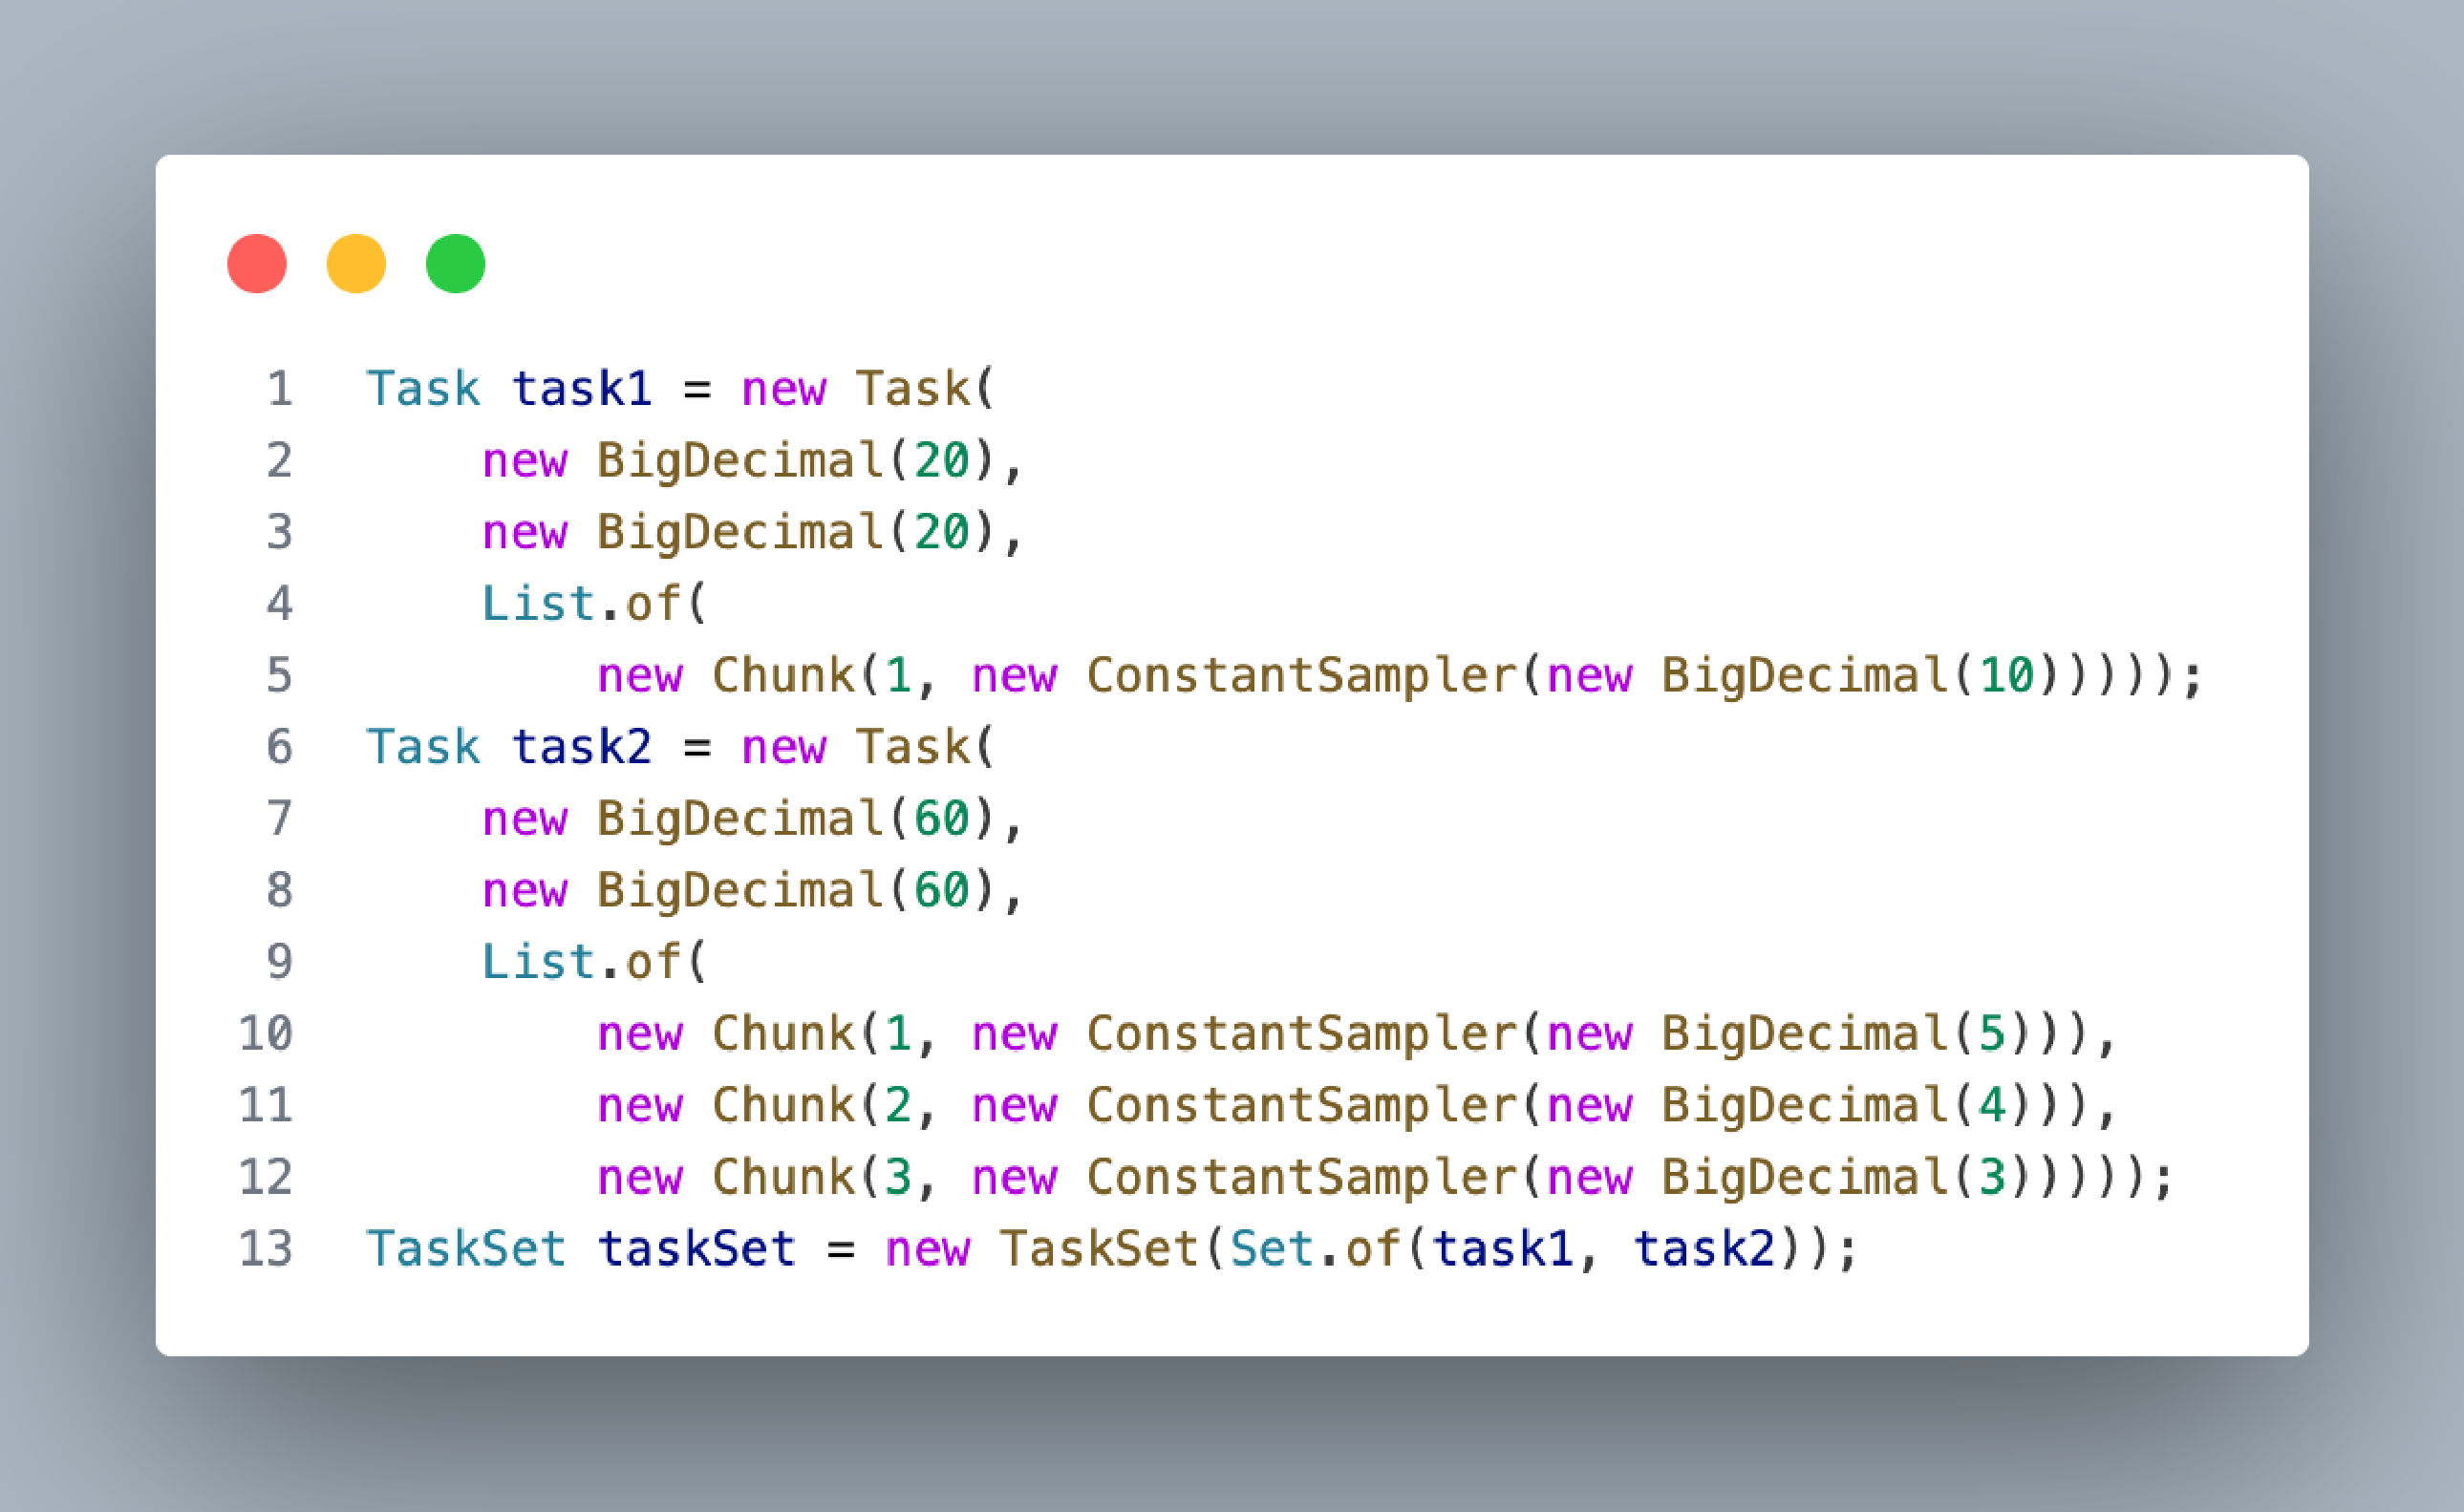
\includegraphics[width=.9\textwidth]{immagini/taskset baseline.pdf}
        }
        \caption{Taskset della baseline}
        \label{fig:baselineTaskset}
        \vfill
    \end{subfigure}
    \hfill
    \begin{subfigure}{0.45\textwidth}
        \vfill
        \centering
        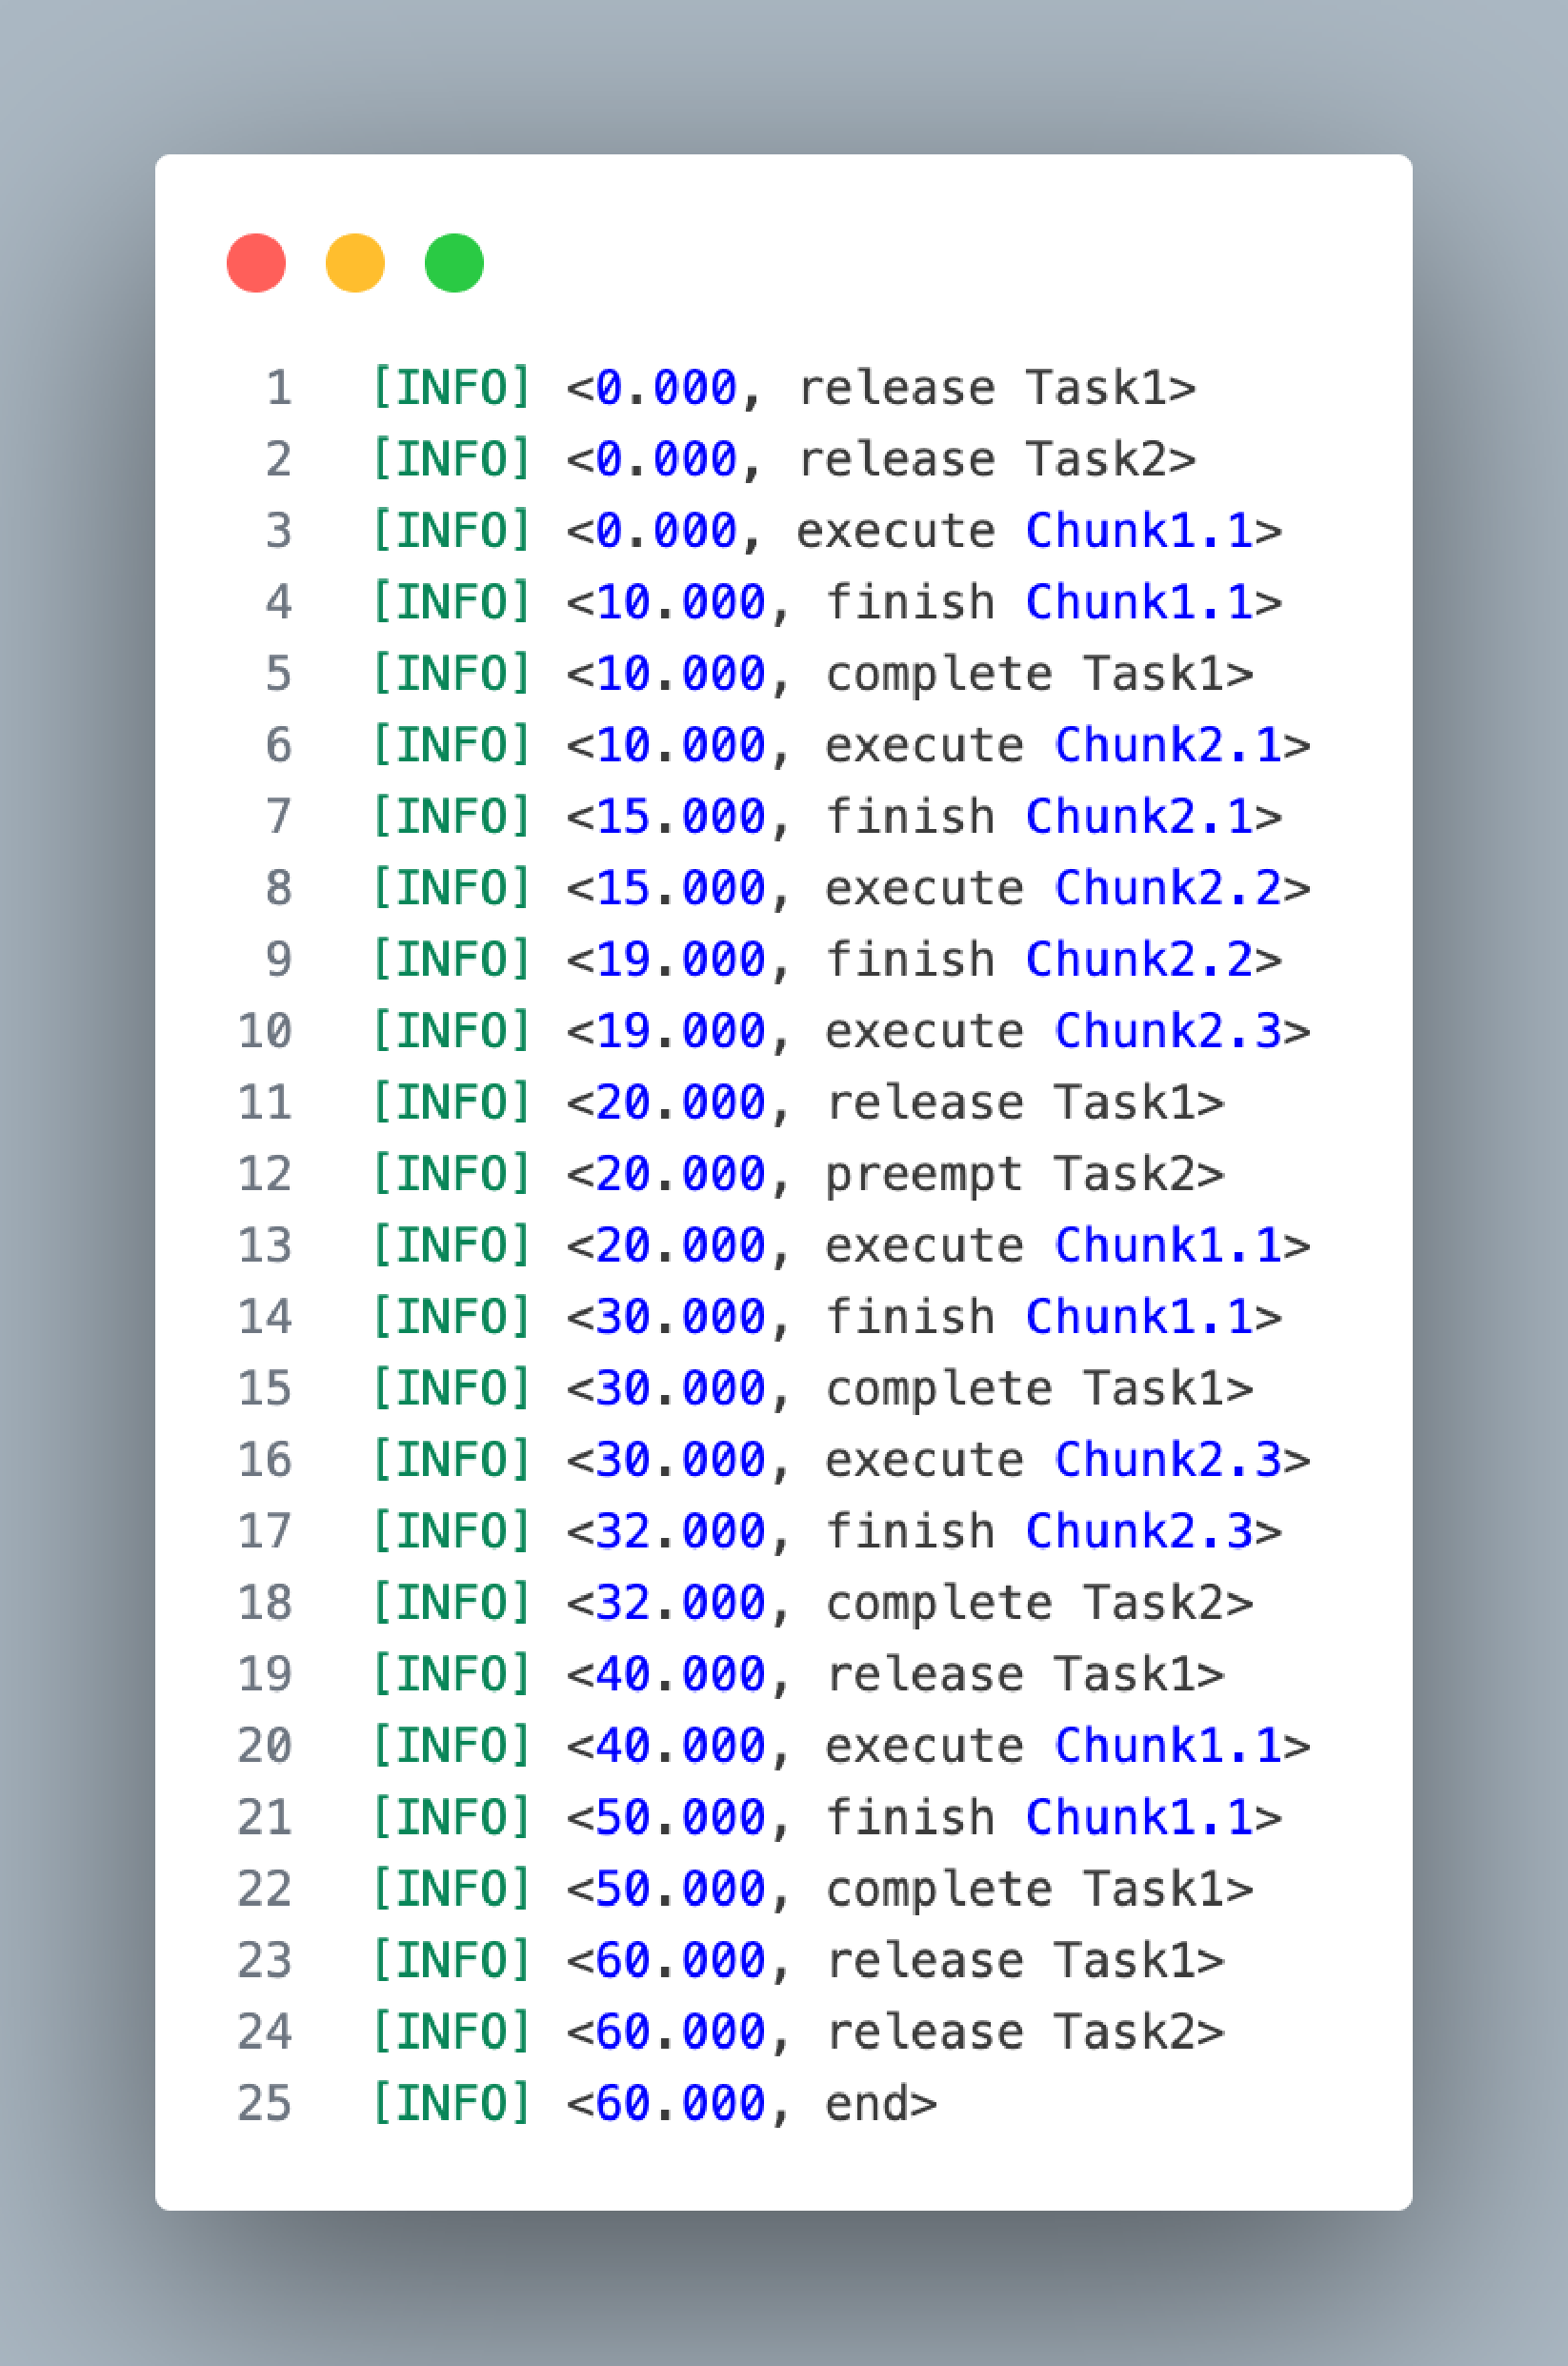
\includegraphics[width=.9\textwidth]{immagini/trace baseline.pdf}
        \caption{Traccia della baseline}
        \label{fig:baselineTrace}
        \vfill
    \end{subfigure}
    \caption{Baseline.}
\end{figure}

\myskip

Di seguito osserviamo invece lo stesso taskset schedulato sempre con RM, ma in cui due chunk (uno per task) condividono una risorsa. In Figura~\ref{fig:baselineTasksetWRes} possiamo osservare come configurarlo, mentre in Figura~\ref{fig:baselineTraceWRes} possiamo osservare la traccia della simulazione.

\begin{figure}[htbp]
    \centering
    \begin{subfigure}{0.45\textwidth}
        \vfill
        \centering
        \raisebox{9em}{
            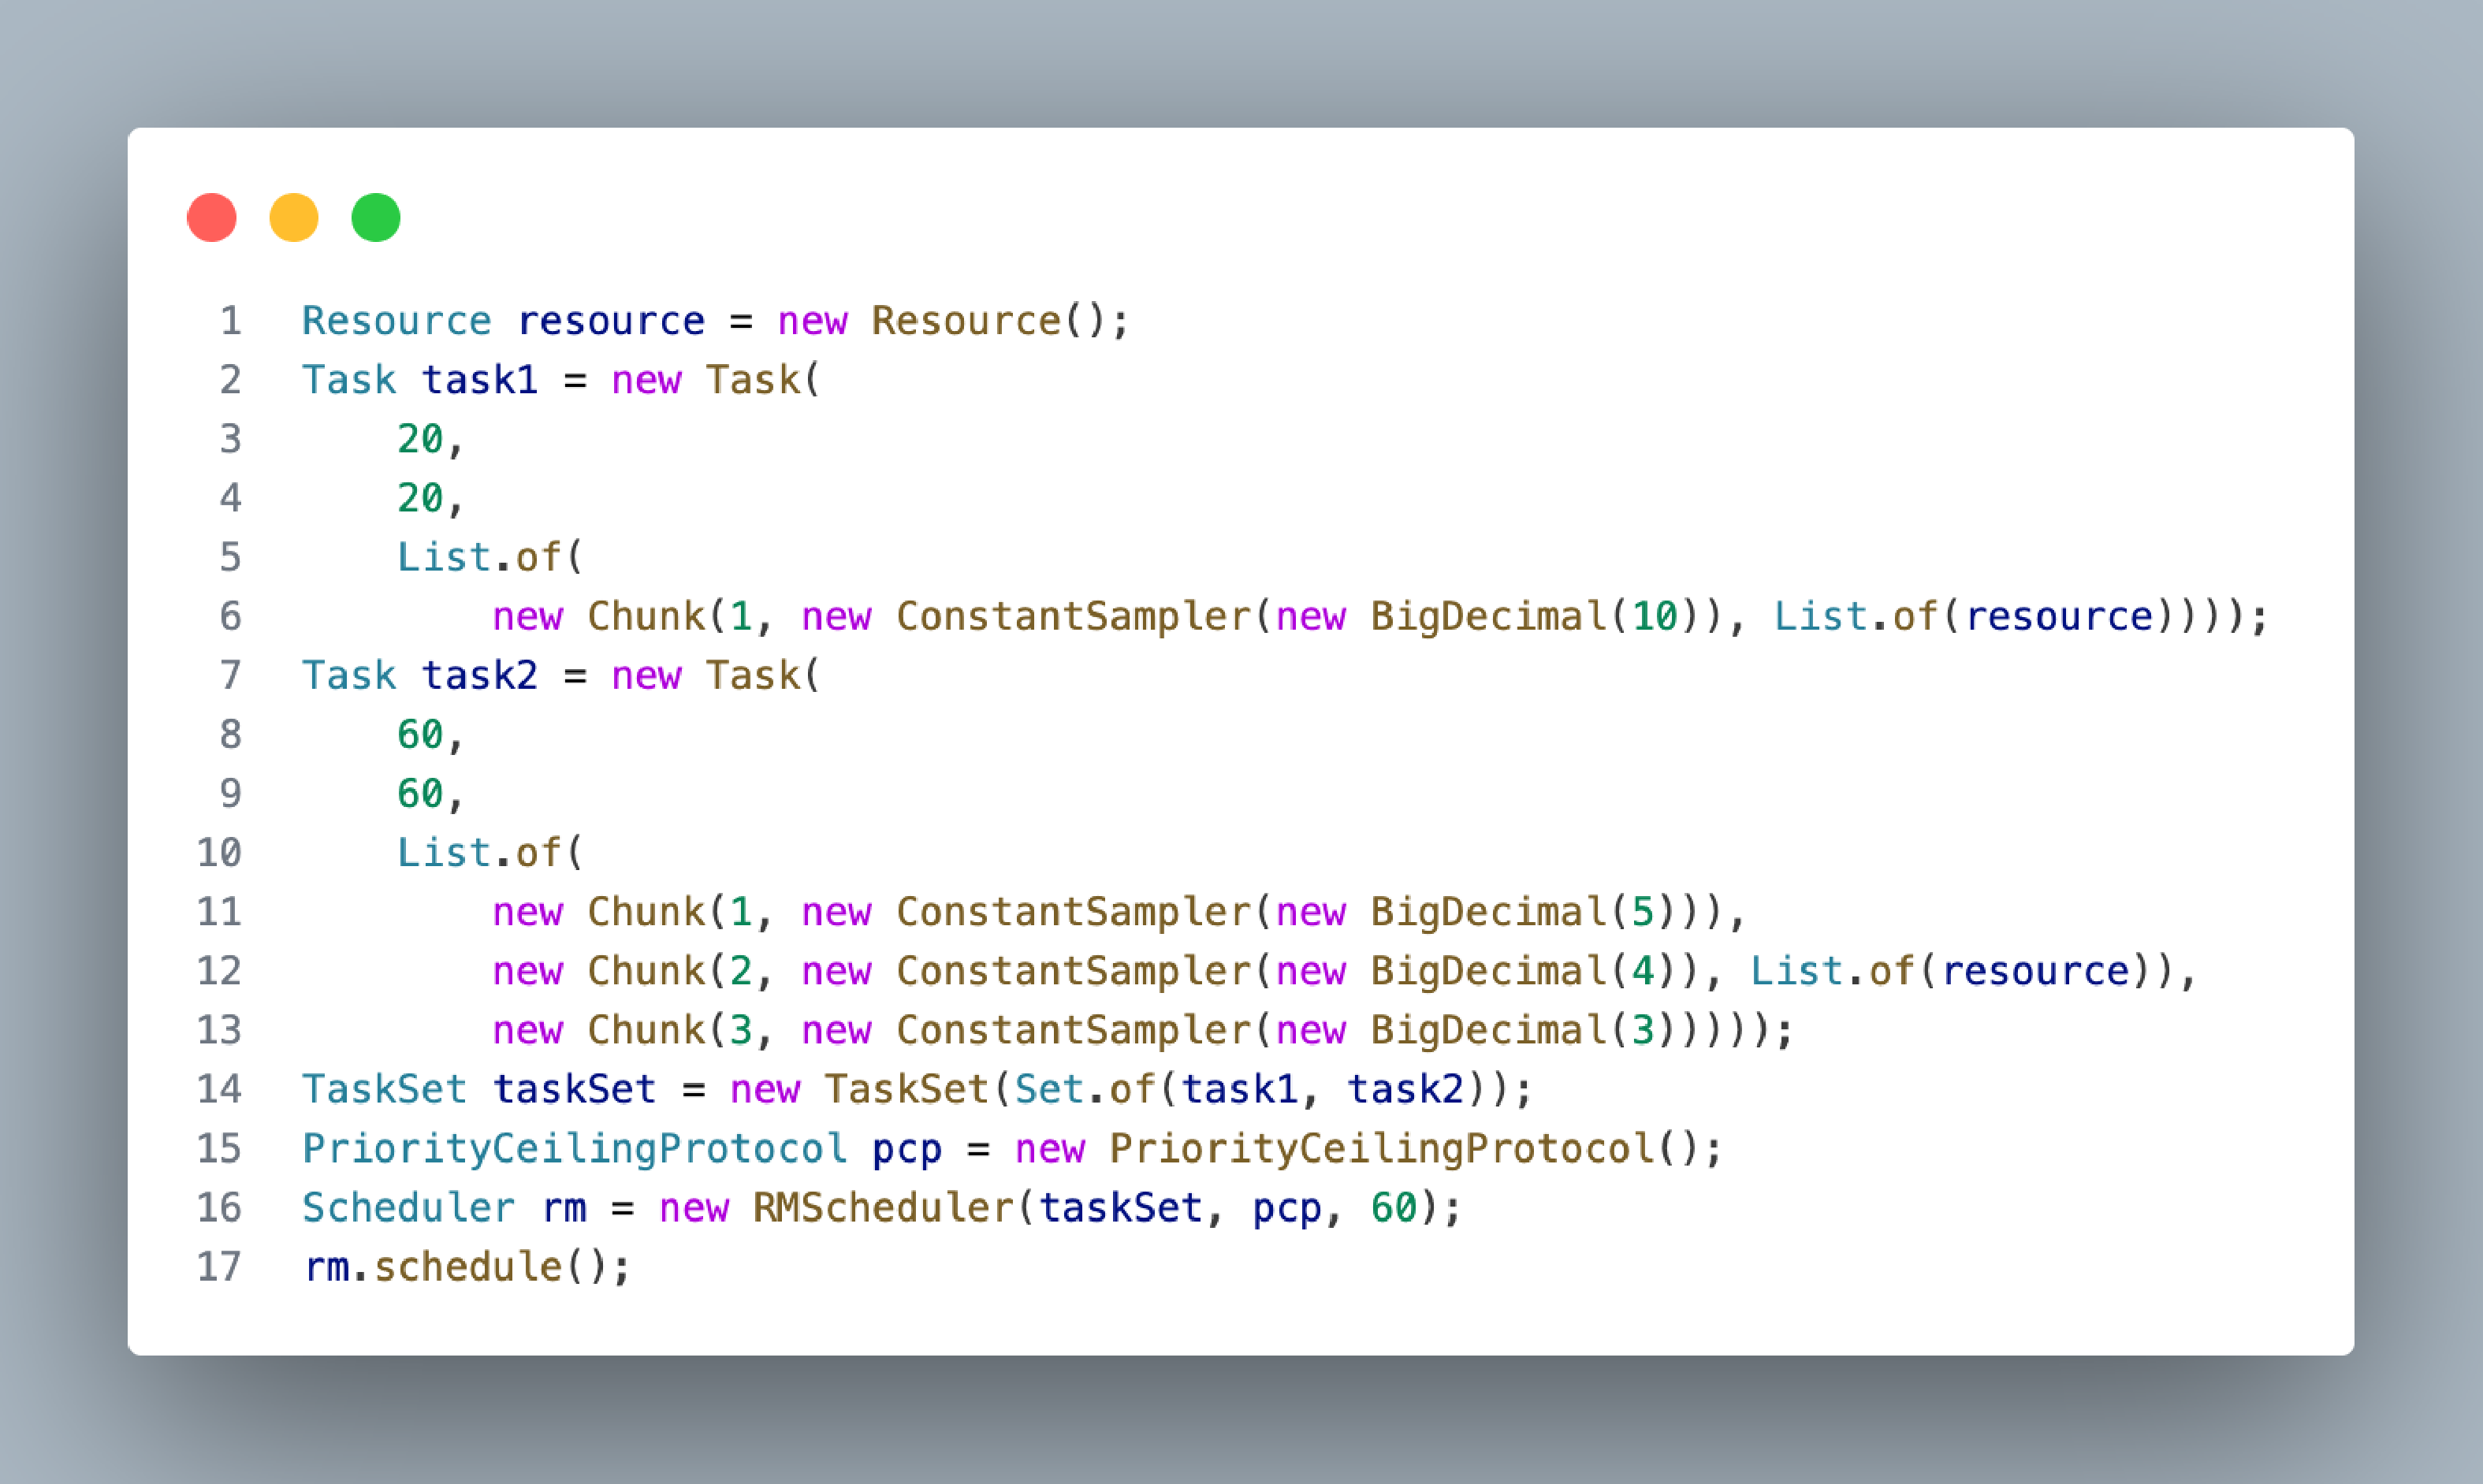
\includegraphics[width=.9\textwidth]{immagini/taskset baseline con risorse.pdf}
        }
        \caption{Taskset della baseline con risorsa condivisa}
        \label{fig:baselineTasksetWRes}
        \vfill
    \end{subfigure}
    \hfill
    \begin{subfigure}{0.45\textwidth}
        \vfill
        \centering
        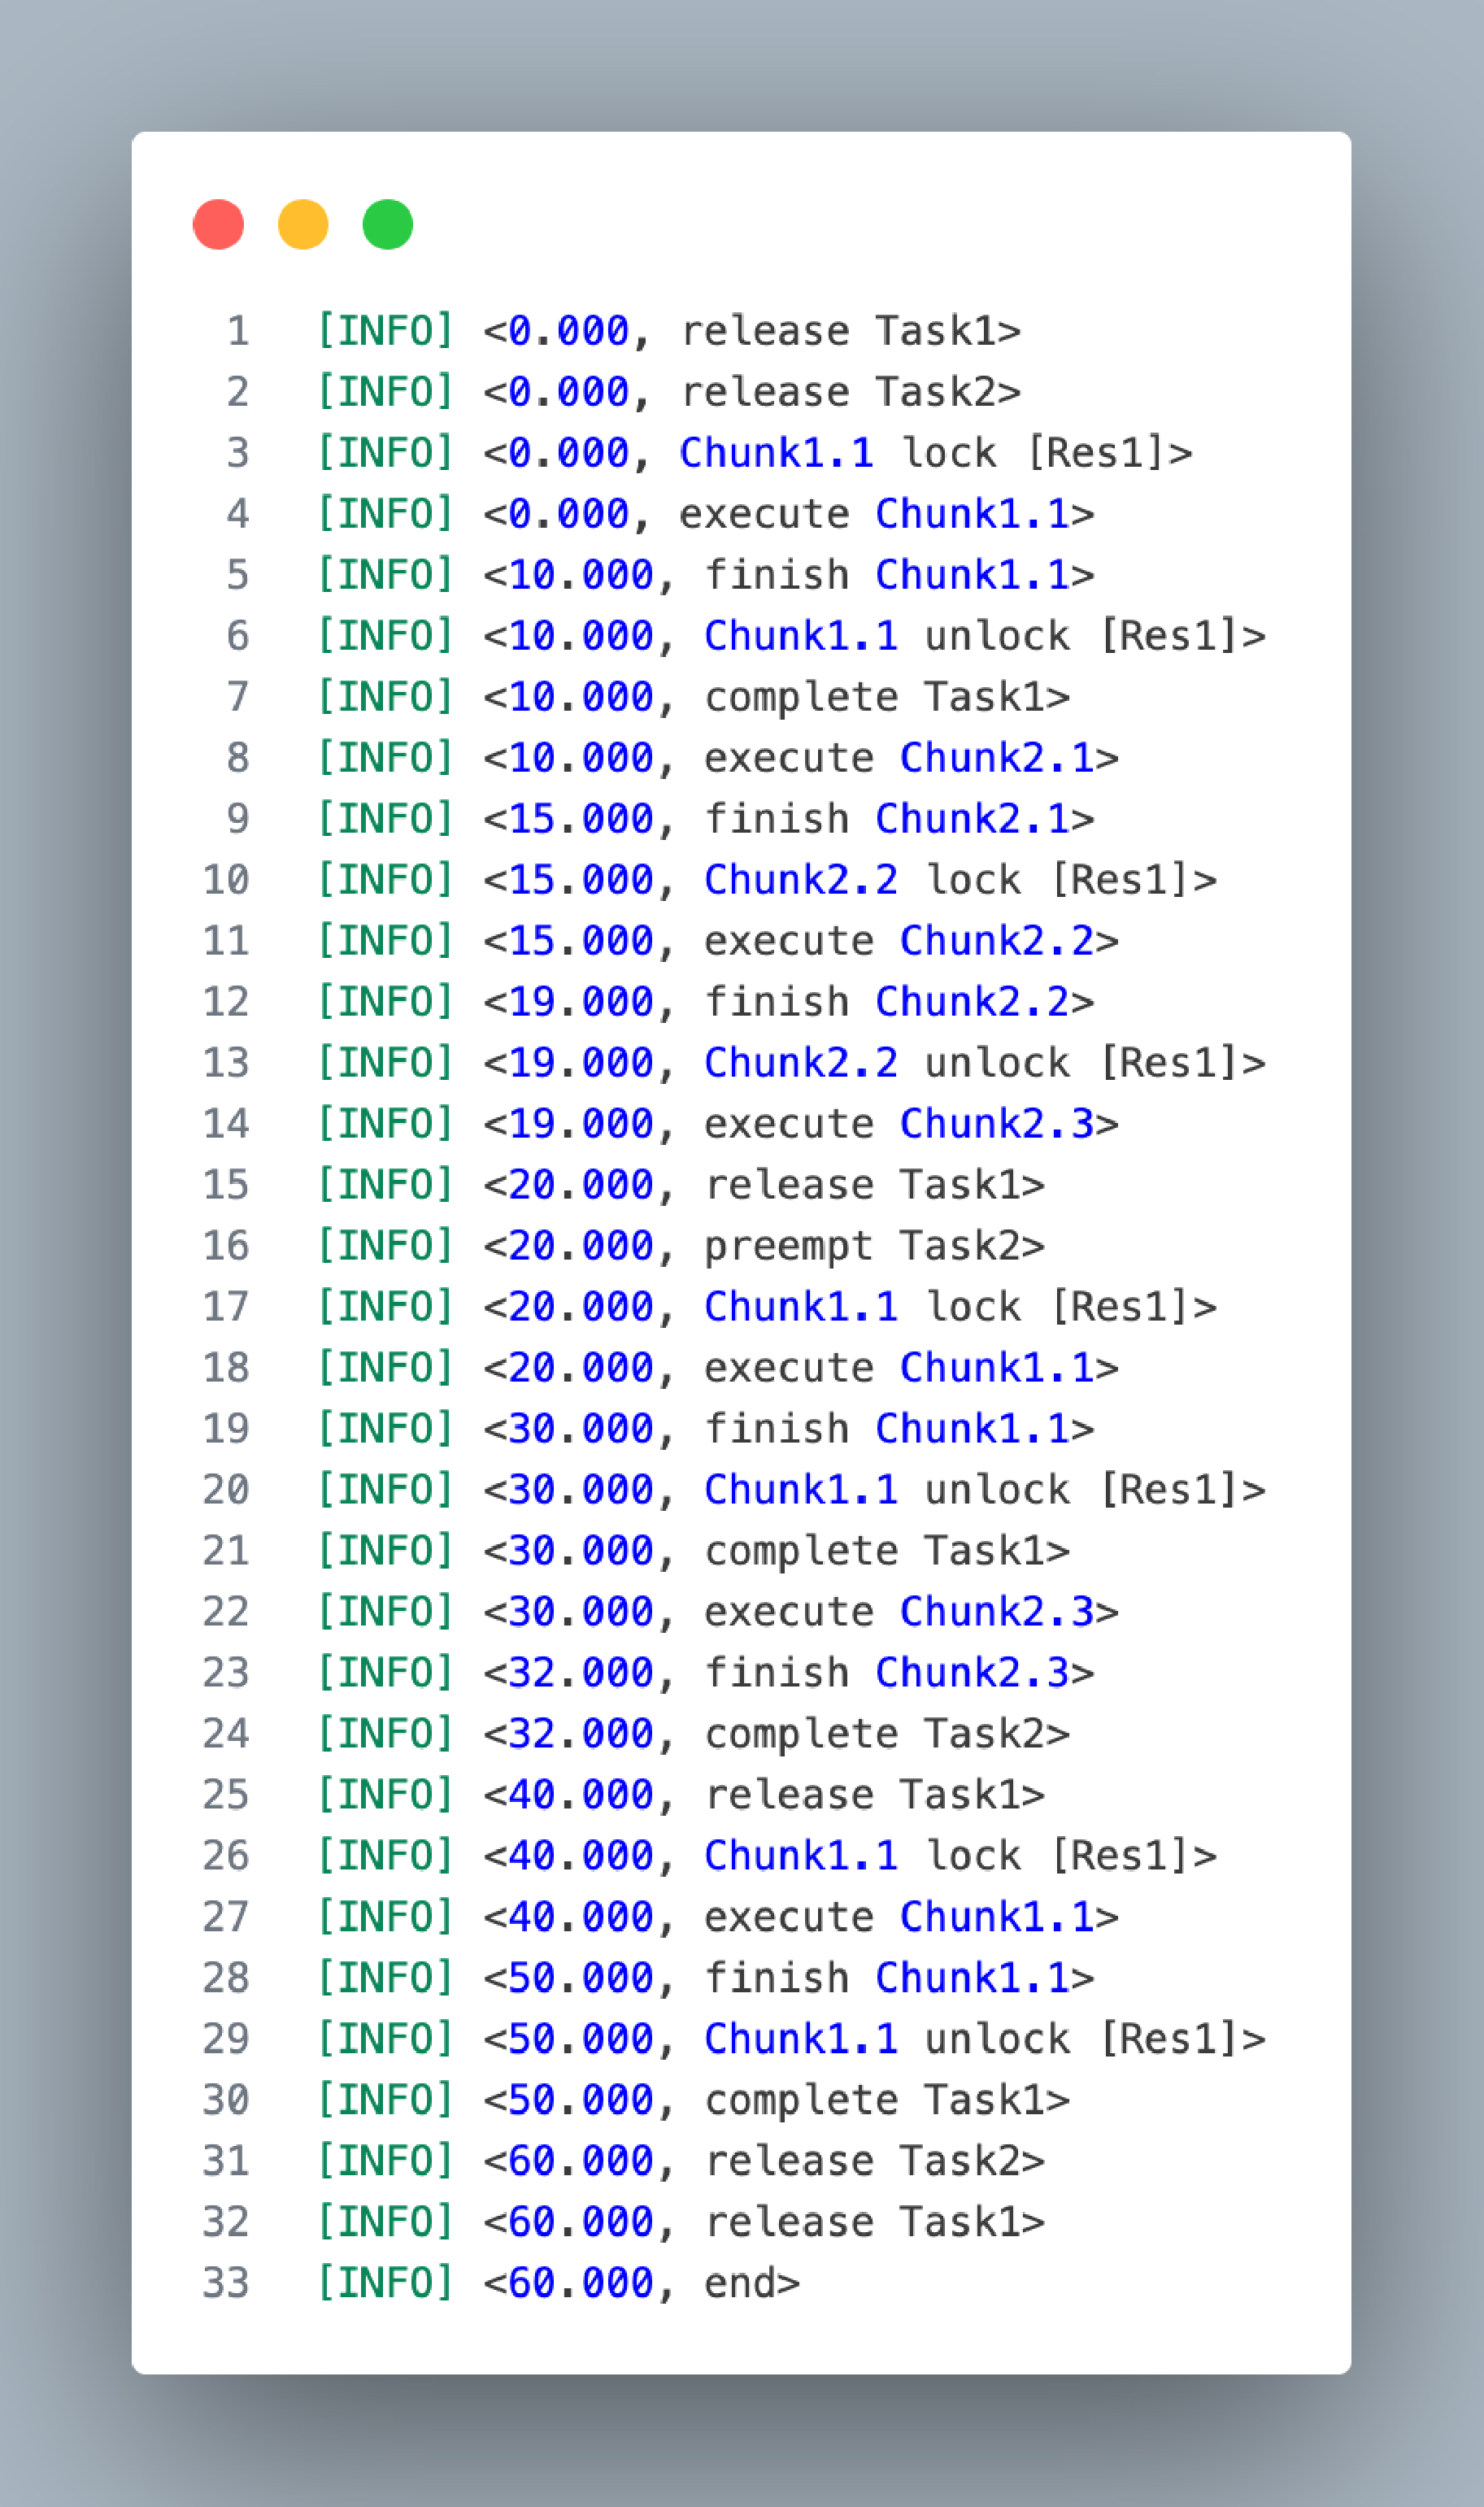
\includegraphics[width=.9\textwidth]{immagini/trace baseline con risorse.pdf}
        \caption{Traccia della baseline con risorsa condivisa}
        \label{fig:baselineTraceWRes}
        \vfill
    \end{subfigure}
    \caption{Baseline con risorsa condivisa}
\end{figure}

%%%%%%%%%%%%%%%%%%%%%%%%%%%%%%%%%%%%%%%%%%%%%%%%%%%%%%%%%%%%%%%%
\section{Chunk additional execution time}
Nella Figura~\ref{fig:tasksetAdditionalET} si osserva come specificare un chunk che campiona un additional execution time da una distribuzione. Nella Figura~\ref{fig:traceAdditionalET} invece si può notare come questo comportamento sia loggato dal sistema. Per osservare questa funzionalità si usa lo stesso taskset della sezione precedente.

\begin{figure}[htbp]
    \centering
    \begin{subfigure}{0.45\textwidth}
        \vfill
        \centering
        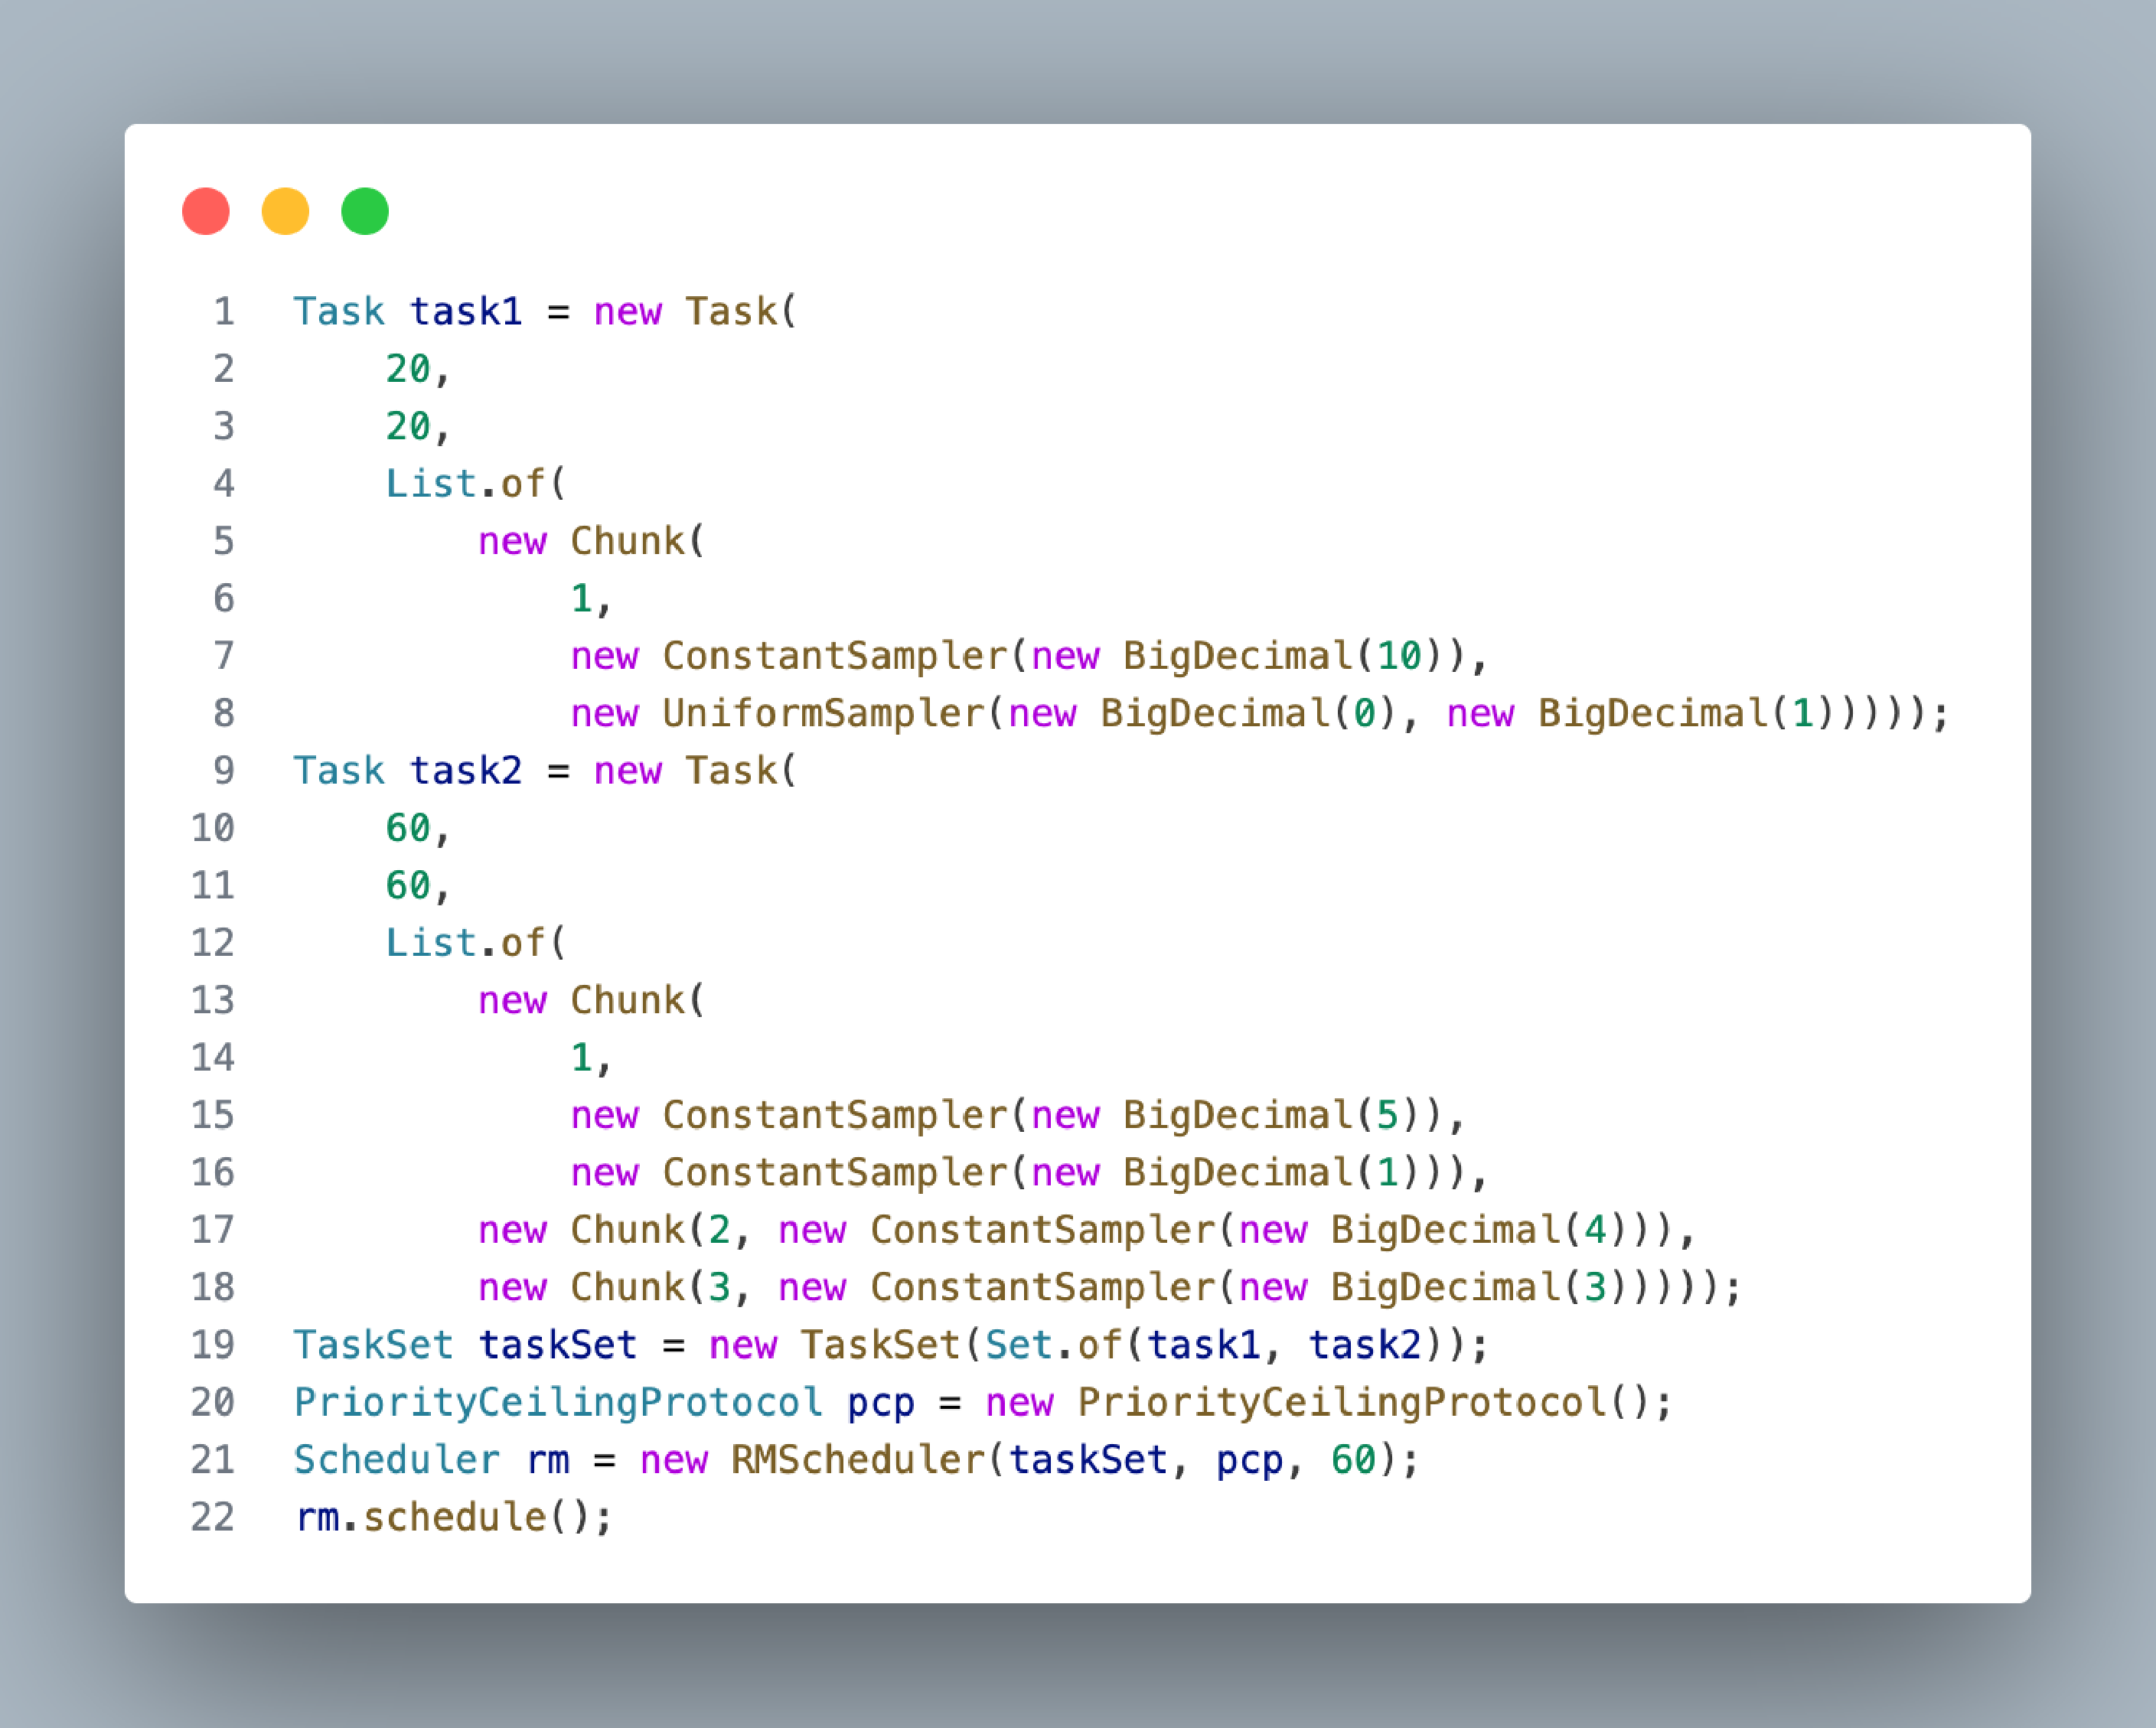
\includegraphics[width=.9\textwidth]{immagini/taskset additional ET chunk.pdf}
        \caption{Taskset con additional execution time}
        \label{fig:tasksetAdditionalET}
        \vfill
    \end{subfigure}
    \hfill
    \begin{subfigure}{0.45\textwidth}
        \vfill
        \centering
        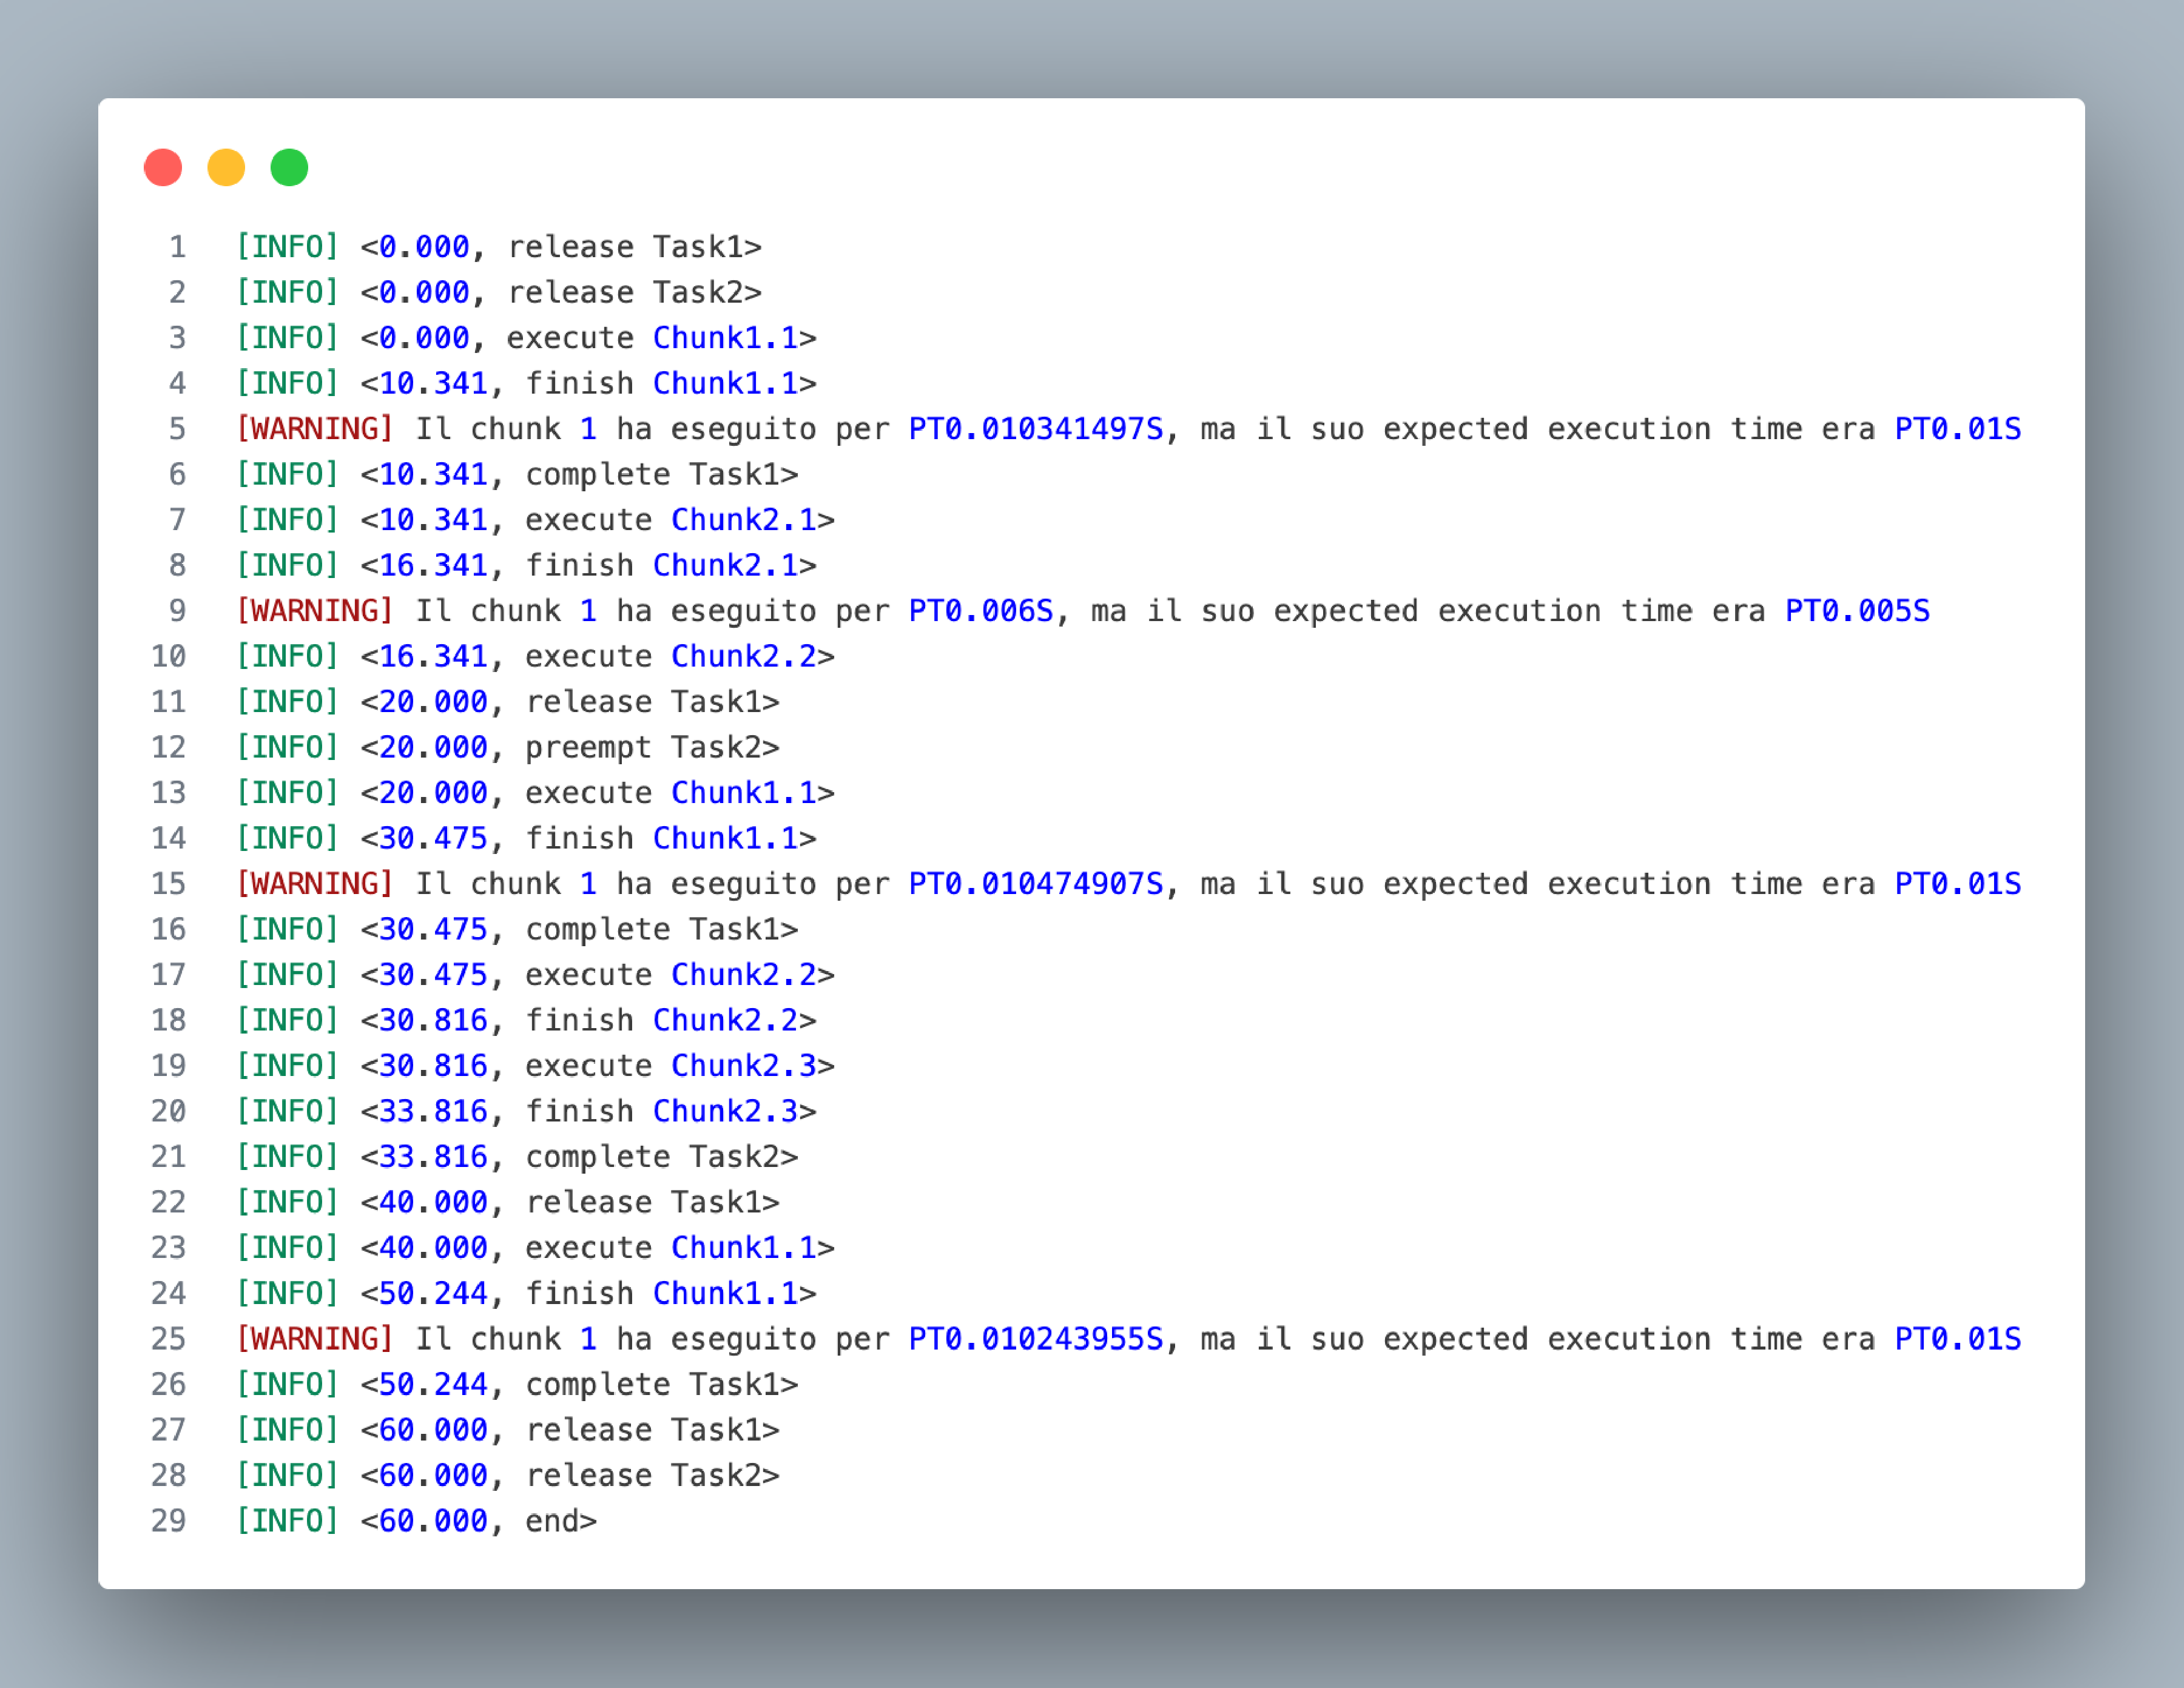
\includegraphics[width=.9\textwidth]{immagini/trace additional ET chunk.pdf}
        \caption{Traccia con additional execution time}
        \label{fig:traceAdditionalET}
        \vfill
    \end{subfigure}
    \caption{Chunk additional execution time}
\end{figure}

%%%%%%%%%%%%%%%%%%%%%%%%%%%%%%%%%%%%%%%%%%%%%%%%%%%%%%%%%%%%%%%%
\section{PCP with faulty priority setting}
Nella Figura~\ref{fig:tasksetFaultSetPriority} vediamo un esempio di simulazione in cui i chunk dei task hanno una risorsa condivisa e il protocollo di accesso alle risorse non si comporta come previsto, ma setta la priorità del task che acquisisce la risorsa pari a quella corretta più un valore campionato da una distribuzione uniforme tra -2 e 2. Questo porta alla generazione della traccia mostrata in Figura~\ref{fig:traceFaultSetPriority}.

\begin{figure}[htbp]
    \centering
    \begin{subfigure}{0.45\textwidth}
        \vfill
        \centering
        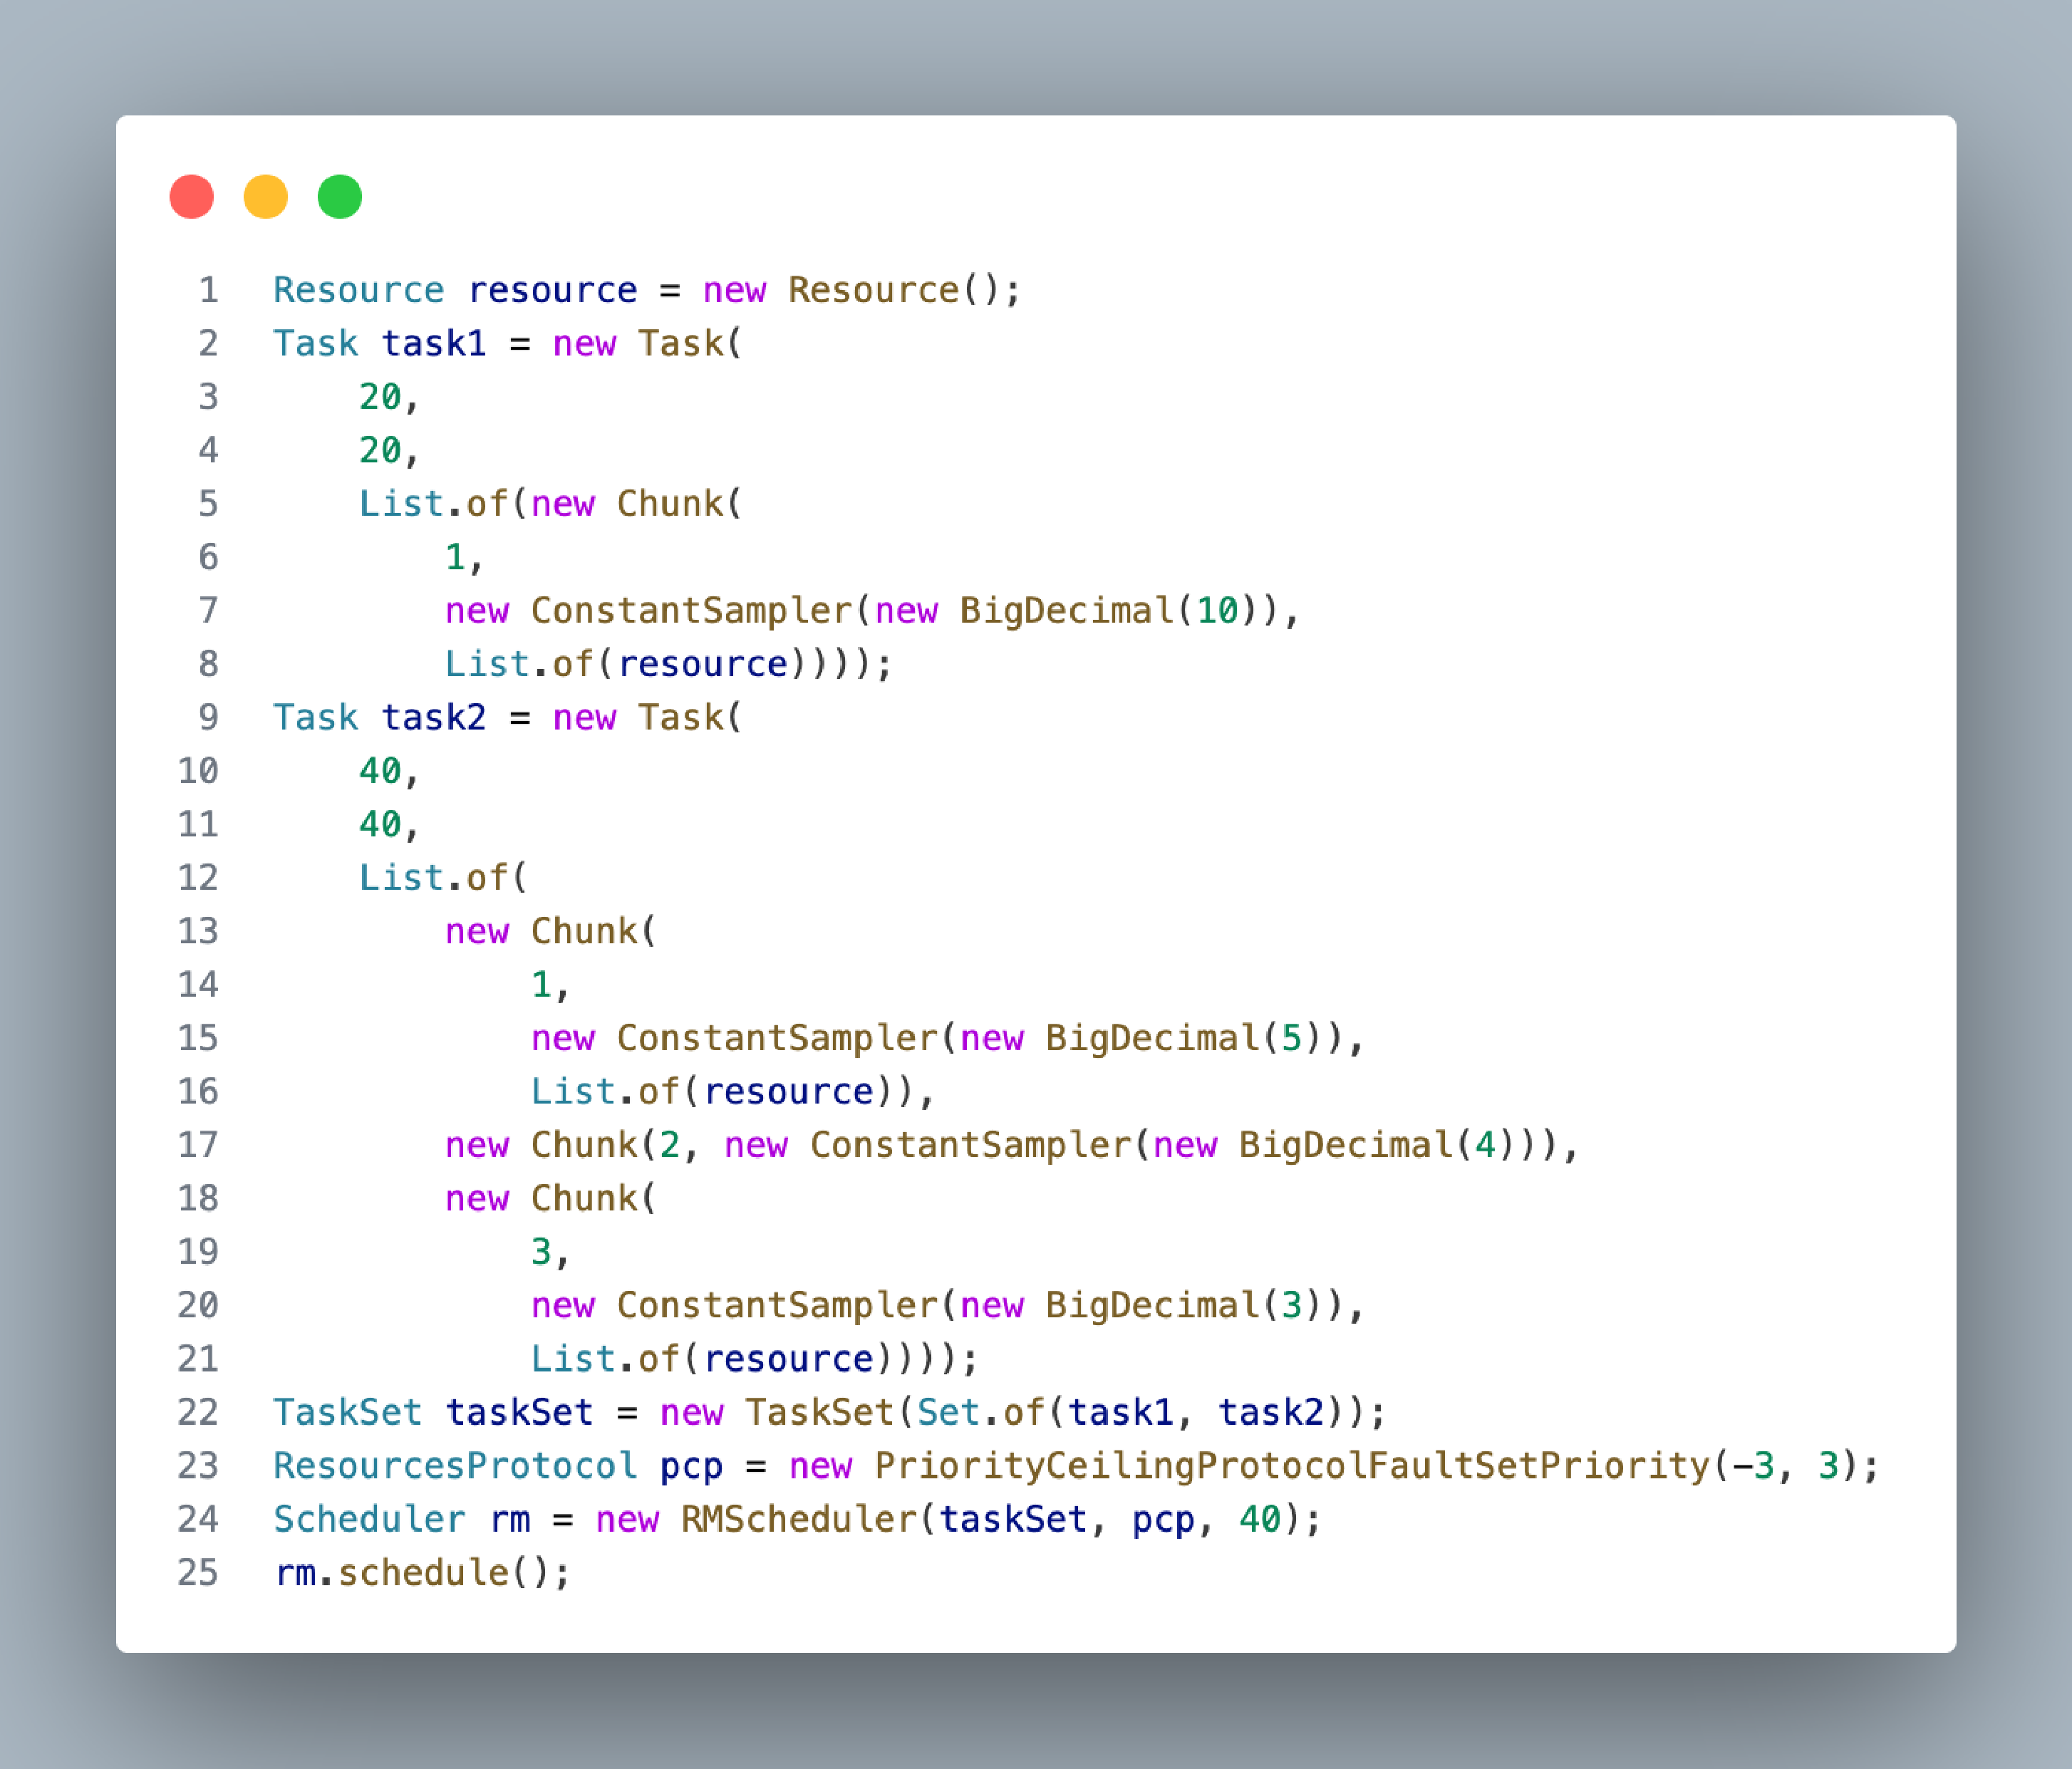
\includegraphics[width=.9\textwidth]{immagini/taskset fault set priority.pdf}
        \caption{Taskset with faulty priority setting}
        \label{fig:tasksetFaultSetPriority}
        \vfill
    \end{subfigure}
    \hfill
    \begin{subfigure}{0.45\textwidth}
        \vfill
        \centering
        \raisebox{1em}{
            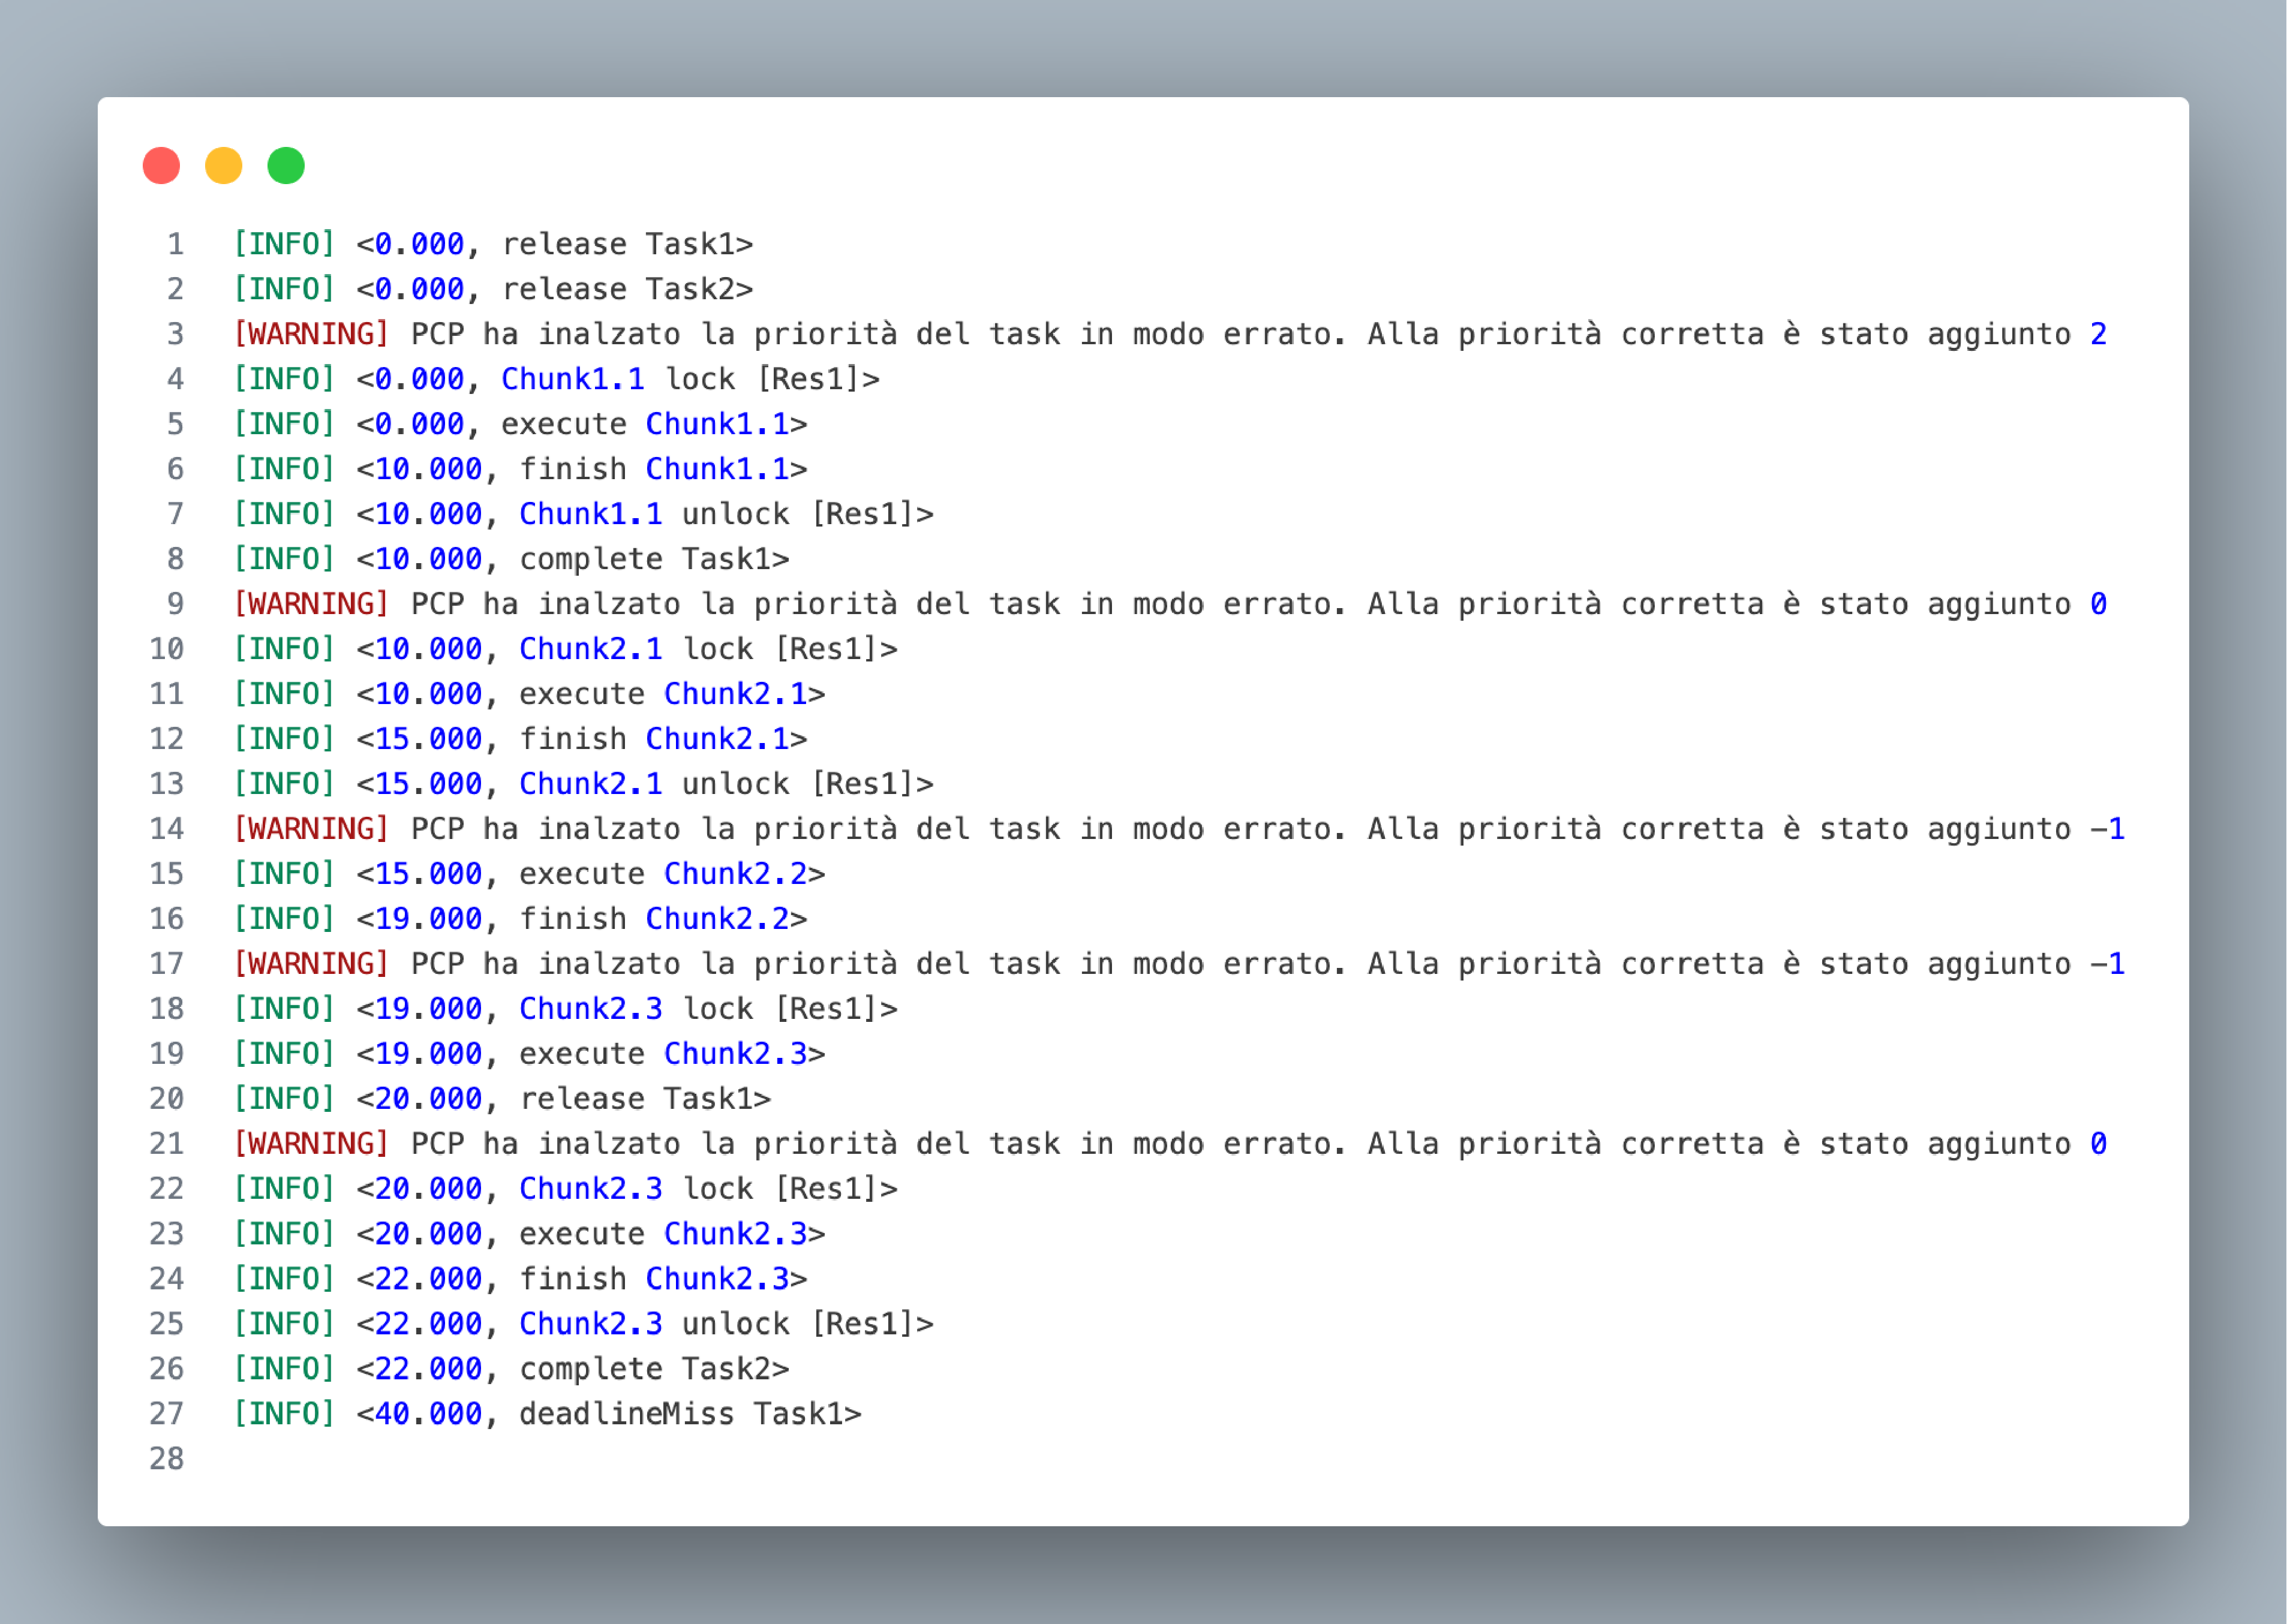
\includegraphics[width=.9\textwidth]{immagini/trace fault set priority.pdf}
        }
        \caption{Trace with faulty priority setting}
        \label{fig:traceFaultSetPriority}
        \vfill
    \end{subfigure}
    \caption{PCP with faulty priority setting}
\end{figure}

%%%%%%%%%%%%%%%%%%%%%%%%%%%%%%%%%%%%%%%%%%%%%%%%%%%%%%%%%%%%%%%%
\section{PCP with faulty acquiring resources}
Facendo riferimento allo stesso taskset della sezione precedente, nella Figura~\ref{fig:tasksetFaultAcquiringResources} è mostrato come iniettare il fault relativo alla mancata acquisizione delle risorse con una data probabilità (nell'esempio il 20\%). In Figura~\ref{fig:traceFaultAcquiringResources} invece è mostrato, come sempre fatto fino a ora, la traccia generata dalla simulazione.

\begin{figure}[htbp]
    \centering
    \begin{subfigure}{0.45\textwidth}
        \vfill
        \centering
        \raisebox{2em}{
            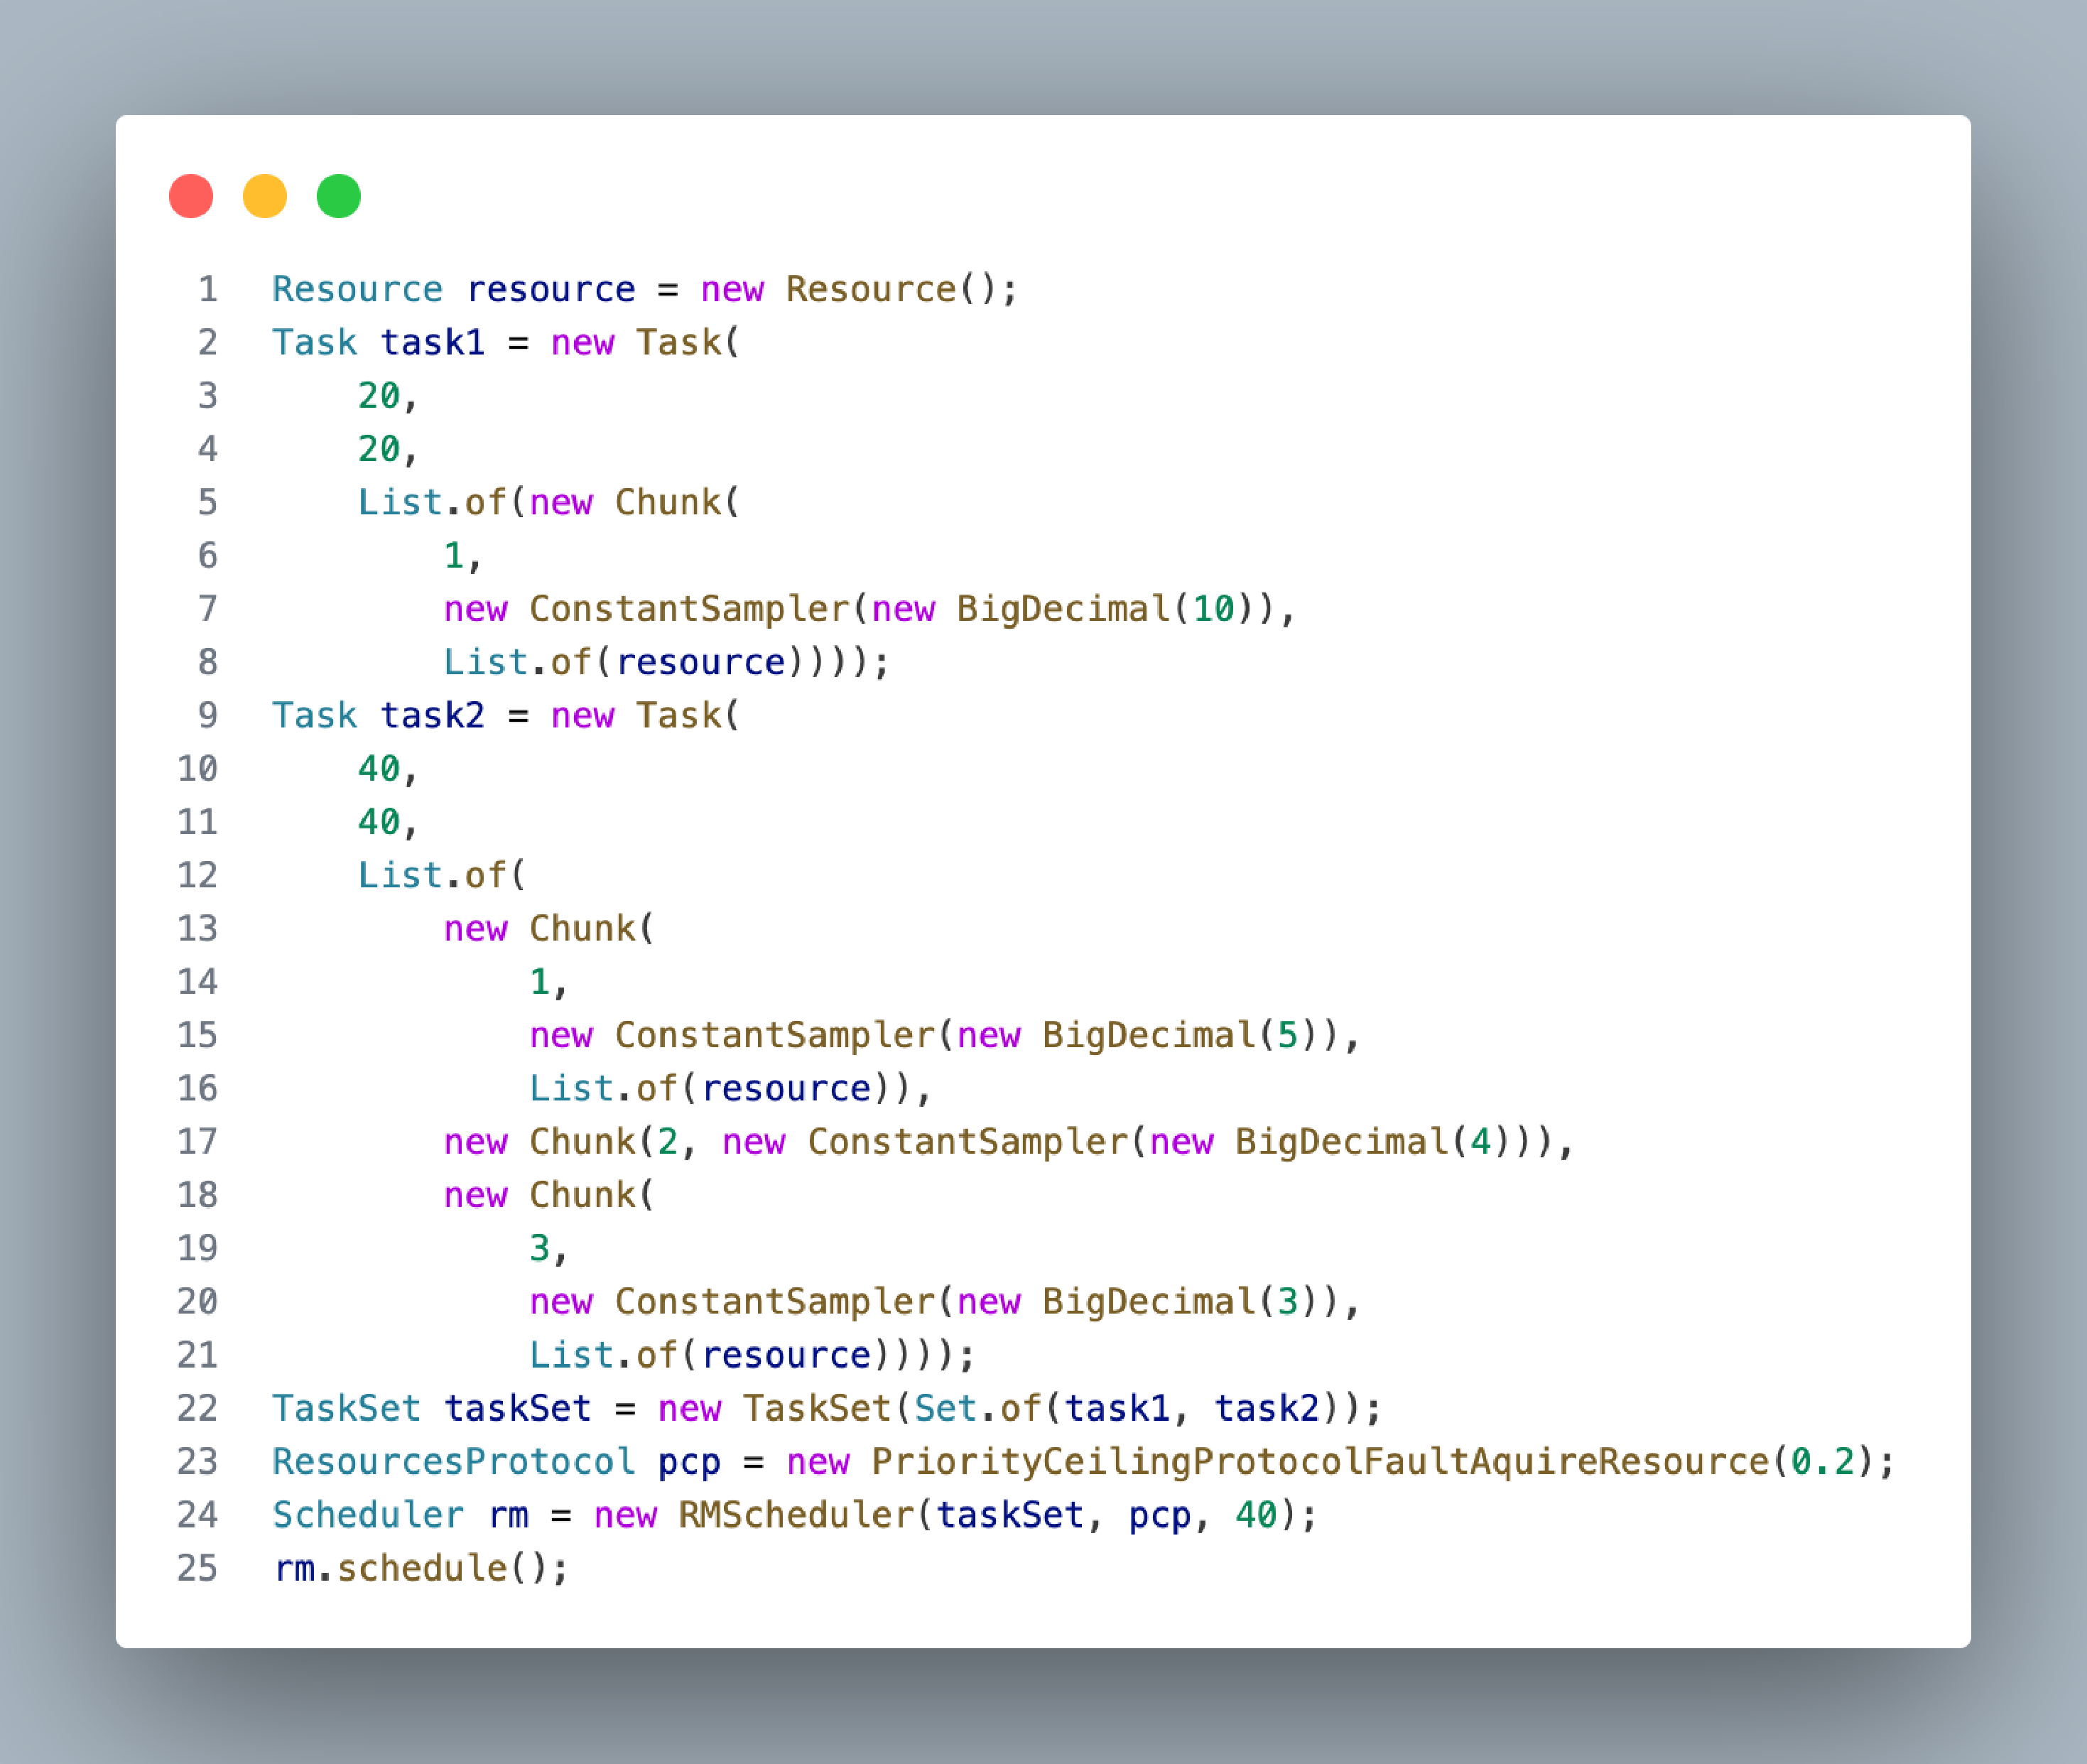
\includegraphics[width=.9\textwidth]{immagini/taskset fault acquire resource.pdf}
        }
        \caption{Taskset with faulty acquiring resources}
        \label{fig:tasksetFaultAcquiringResources}
        \vfill
    \end{subfigure}
    \hfill
    \begin{subfigure}{0.45\textwidth}
        \vfill
        \centering
        \raisebox{1em}{
            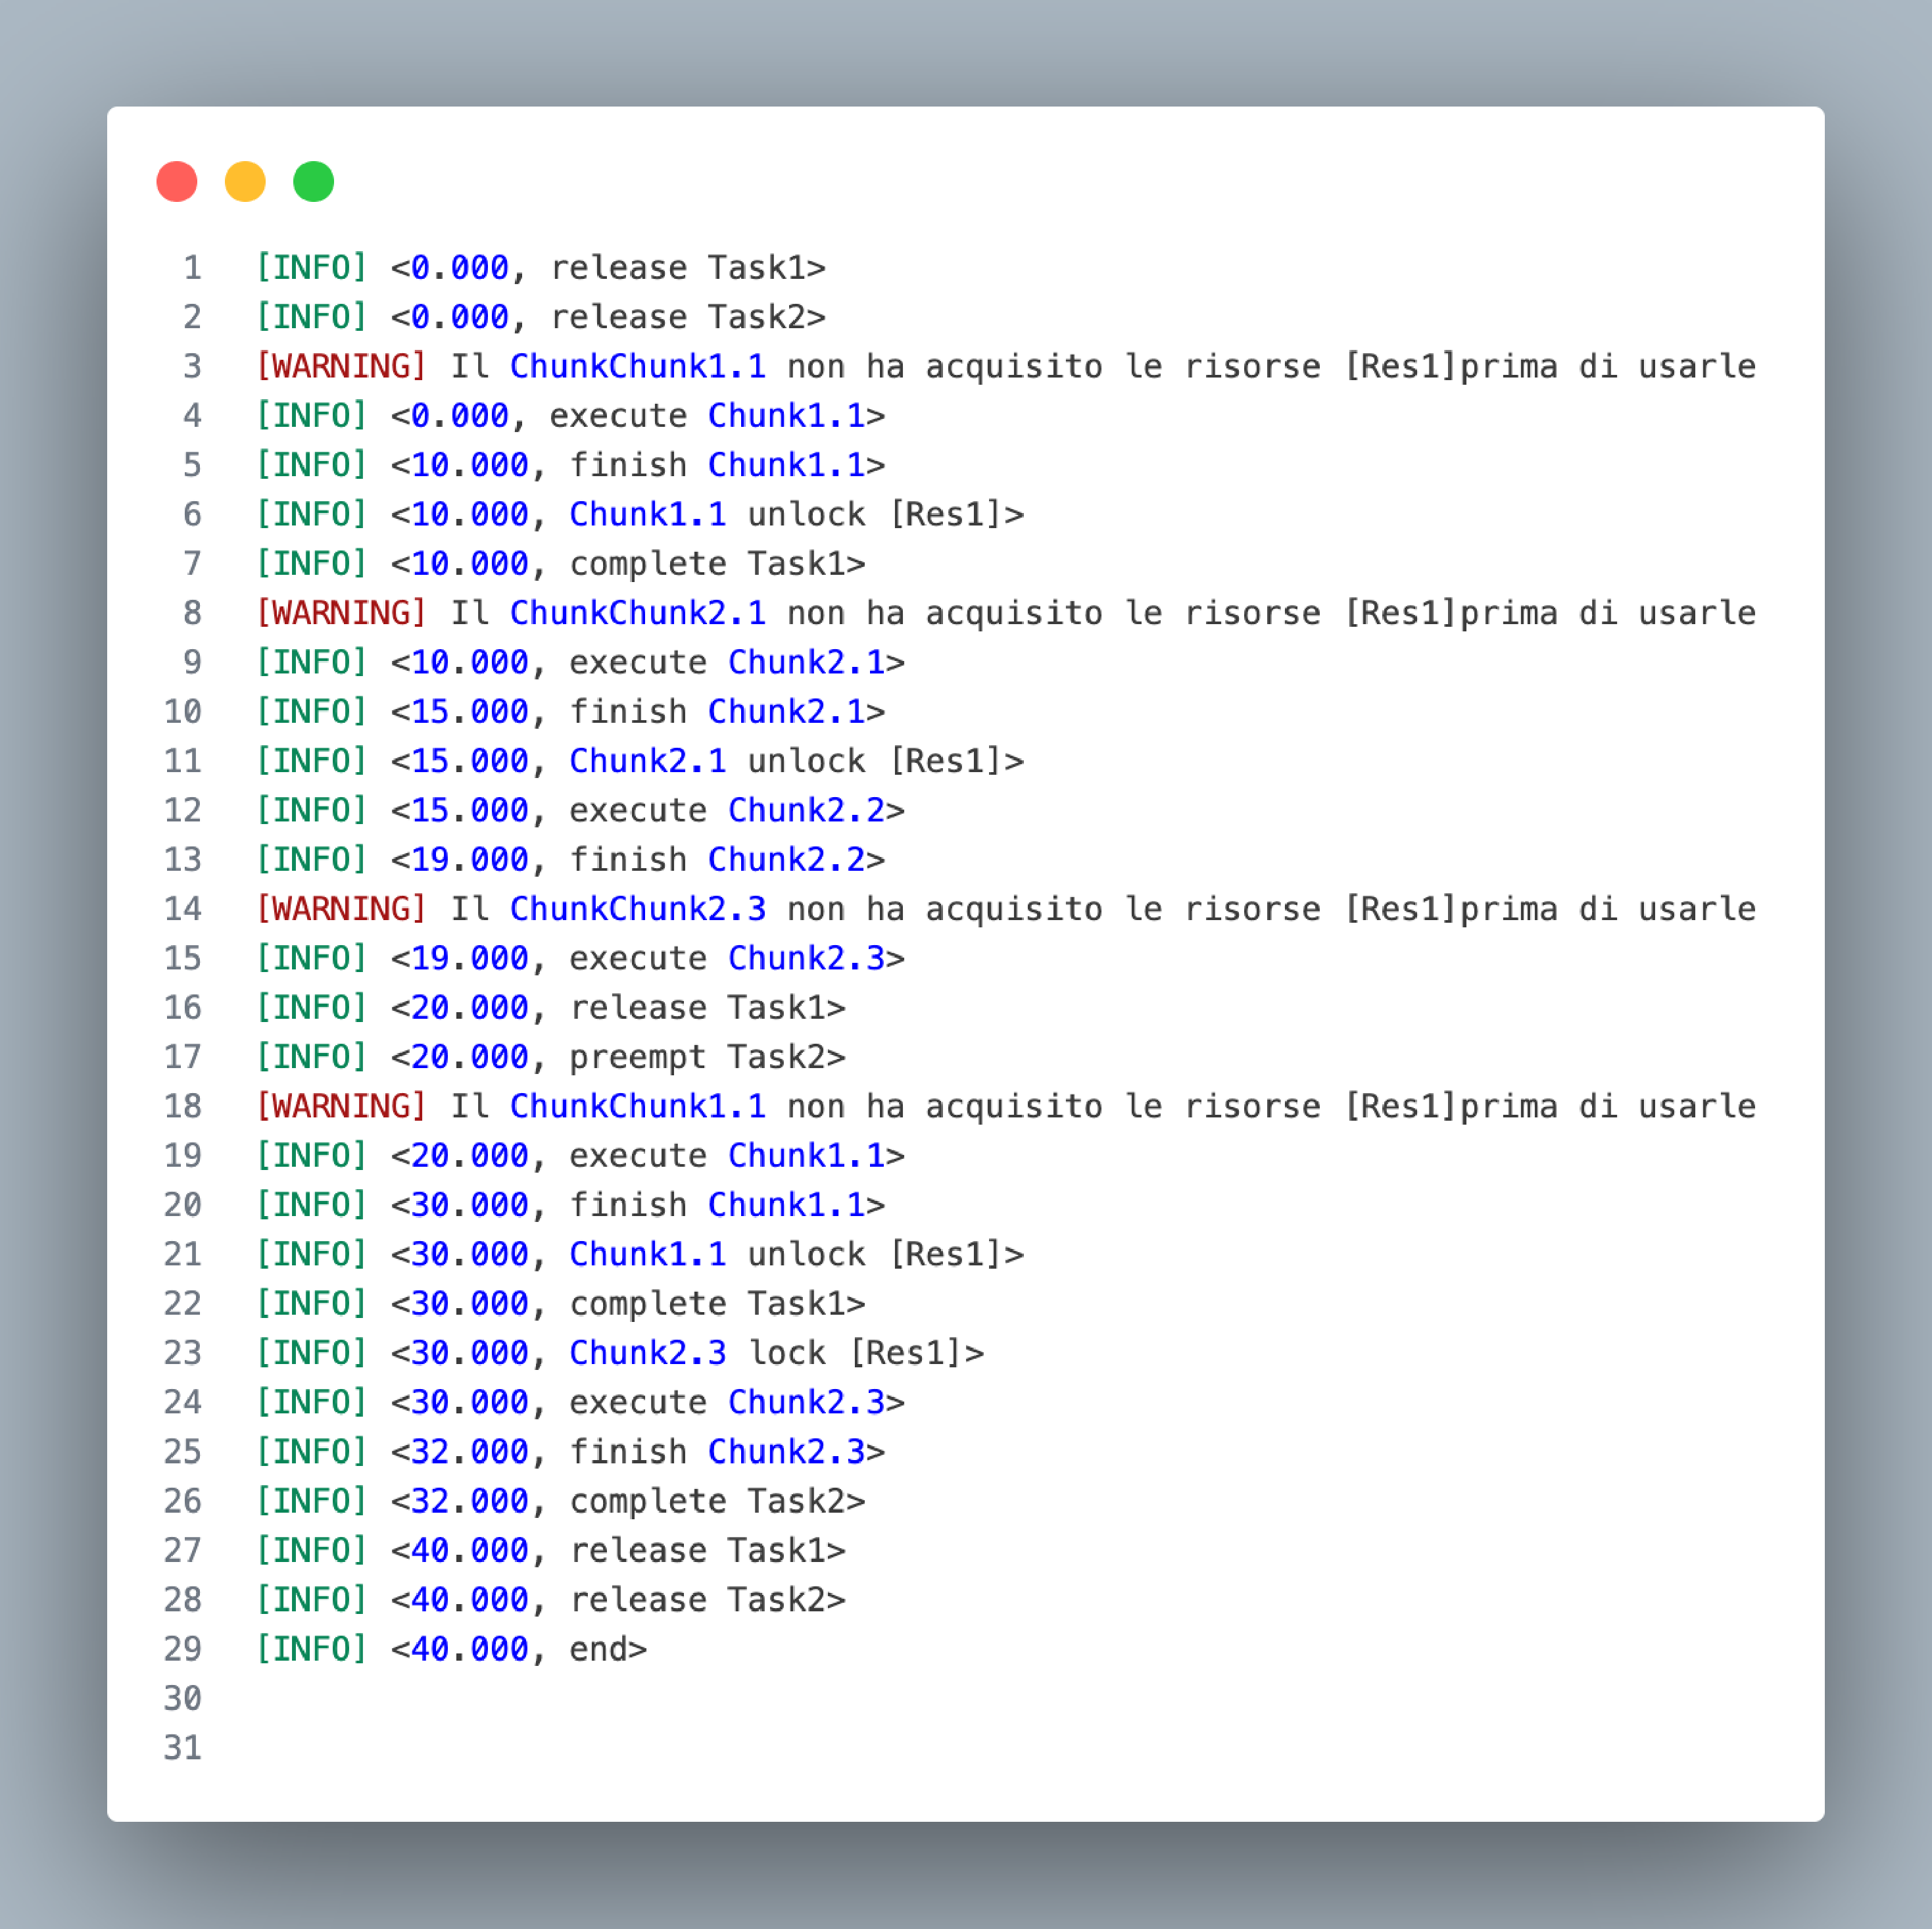
\includegraphics[width=.9\textwidth]{immagini/trace fault acquire resource.pdf}
        }
        \caption{Trace with faulty acquiring resources}
        \label{fig:traceFaultAcquiringResources}
        \vfill
    \end{subfigure}
    \caption{PCP with faulty acquiring resources}
\end{figure}